\chapter{Radiaci\'{o}n de Hawking an\'{a}loga en sistemas \'{o}pticos}\label{cap4}
Desde un punto de vista práctico, la luz en medios diel\'{e}tricos proporciona un atractivo sistema experimental para observar la radiación de Hawking an\'{a}loga. Sin embargo, en estos sistemas el medio no se mueve, entonces ¿c\'{o}mo se crea en este caso un horizonte?, ¿es necesario mover físicamente un medio para establecer un horizonte? Recordemos que la existencia de un horizonte es uno de los ingredientes esenciales para que exista el proceso de Hawking. En el caso de los an\'{a}logos \'{o}pticos, lo que realmente importa son solo las propiedades efectivas del medio que indican c\'omo se propagan las ondas en el interior del material.\\

Tales ideas se pueden discutir desde el marco de la \'{o}ptica no lineal, particularmente como un pulso de luz muy intenso al propagarse en el interior de una fibra \'{o}ptica modifica sus propiedades ópticas debido al efecto Kerr \'{o}ptico \citep{Agrawal2013}. El índice de refracción original de la fibra $n_{0}$ gana una contribución adicional $\delta n$ que es proporcional a la intensidad $I$ del pulso, pero como el pulso se mueve a trav\'{e}s del material, esta contribución al $n_{0}$ se mover\'{a} a la misma velocidad estableciendo así un medio en movimiento, aunque no se desplaza nada material. Este medio efectivo se mueve naturalmente a la velocidad de la luz dentro de la fibra, porque está hecho por luz misma.\\

En este cap\'{i}tulo haremos un an\'{a}lisis similar al expuesto en el cap\'{i}tulo \ref{cap2}, encontrando la ecuaci\'{o}n din\'{a}mica que sigue un campo cu\'{a}ntico cuando se propaga en el interior de una fibra \'{o}ptica, posteriormente linealizaremos la ecuaci\'{o}n diferencial que rige la din\'{a}mica de este campo para ver la relaci\'{o}n de dispersi\'{o}n para una fluctuaci\'{o}n que se propaga sobre dicho campo. Por \'{u}ltimo, explicaremos la idea de horizontes en \'{o}ptica para concluir con el sistema de l\'{a}ser \'{o}ptico de agujeros negros.

\section{\'{O}ptica no lineal}
La \'{o}ptica no lineal estudia la respuesta de los medios dieléctricos a campos ópticos. Cuando la intensidad de los campos es lo suficientemente alta, la respuesta del medio es no lineal, i.e., la polarización, que es el momento dipolar por unidad de volumen en el medio, no es una función lineal del campo eléctrico aplicado. En la descripci\'{o}n de la polarización hay un término lineal pero tambi\'{e}n términos que contienen  potencias mayores del campo eléctrico que conducen a nuevos tipos de comportamiento. Uno de los más notables es que las frecuencias de estos nuevos campos sean arm\'{o}nicos de la frecuencia del campo de entrada. Los medios lineales no cambian la frecuencia de la luz que incide sobre ellos, de hecho, la primera observación de un efecto óptico no lineal fue la generación del segundo armónico \citep{franken1961generation}, donde un haz de luz láser que entra en un medio no lineal produce un segundo haz al doble de la frecuencia del original. Otro tipo de comportamiento que se hace posible en medios no lineales es que el índice de refracción sea una función de la intensidad de la luz y de la frecuencia, lo que permite construir un medio m\'{o}vil an\'{a}logo a un fluido en movimiento y as\'{i} reproducir las ideas mencionadas en los cap\'{i}tulos \ref{cap2} y \ref{cap3}.\\

La mayoría de los efectos ópticos no lineales se pueden describir utilizando campos electromagnéticos clásicos, y
de hecho, la teoría inicial de la óptica no lineal se realizó con campos clásicos \citep{armstrong1962interactions}. Sin embargo, cuando los campos se cuantizan surgen una serie de nuevos efectos. Los campos cuantizados son necesarios para describir radiaci\'{o}n que se origina a partir de la \textit{emisión espontánea}. Por ejemplo, en un proceso conocido como conversión descendente paramétrica espontánea o en ingl\'{e}s \textit{spontaneous parametric down conversion} (SPDC), un fot\'{o}n atraviesa un cristal no lineal y en el proceso se producen un par de fotones a la mitad de la frecuencia del original debido a una emisión espontánea. Por otro lado, el efecto Hawking es una emisi\'{o}n espont\'{a}nea, por tanto requiere que la descripci\'{o}n de los campos sea cu\'{a}ntica.\\

Cuando un campo el\'{e}ctrico es aplicado a un medio diel\'{e}ctrico, una polarizaci\'{o}n es creada en el medio. Las ecuaciones de Maxwell para materiales no magn\'{e}ticos en ausencia de cargas y corrientes externas que incluyen la polarizaci\'{o}n son

\begin{align}\label{ec:Maxwells}
\nabla \cdot \textbf{D}&=0, \hspace{2cm} \nabla \times\textbf{E}=-\partial_t\textbf{B},\\
\nabla\cdot\textbf{B}&=0, \hspace{2cm} \nabla \times \textbf{B}=\mu_0\partial_t \textbf{D},
\end{align}
aqu\'{i} $\textbf{D}=\epsilon_0\textbf{E}+\textbf{P}$ es el campo de desplazamiento y $\textbf{P}$ la polarizaci\'{o}n, i.e., un momento dipolar por unidad de volumen y es dado por 
\begin{equation}\label{ec:polarizacion}
\textbf{P}=\epsilon_0\Bigl[\chi^{(1)}\cdot\textbf{E}+\chi^{(2)}:\textbf{EE}+\chi^{(3)}\vdots\textbf{EEE}+...\Bigr].
\end{equation}
Si las no linealidades en el medio son de origen electrónico, entonces los efectos no lineales deberían ser importantes cuando el campo aplicado es del mismo orden que el campo eléctrico de un átomo. El campo en un átomo $E_{\text{\'{a}tomo}}\thicksim e/(4\pi\epsilon_0 a_0^2)$, donde $a_0$ es el radio de Bohr, el cual es aproximadamente  $5\times10^{11}V/m$. Esto puede usarse para estimar el tama\~{n}o de las susceptibilidades  $\chi^{(i)}$, para campos de esta magnitud los términos en la expansión para la polarización serán de aproximadamente el mismo tamaño. Utilizando el hecho de que $\chi^{(1)}$ es de orden $1$, entonces se encuentra que:
\begin{align}
\chi^{(2)}&\thicksim \frac{1}{E_{\text{\'{a}tomo}}}\approx 2\times10^{-12}\frac{m}{V},\\
\chi^{(3)}&\thicksim \frac{1}{E_{\text{\'{a}tomo}}^2}\approx 4\times10^{-24}\frac{m^2}{V^2}.
\end{align}

La ecuaci\'{o}n de onda cuando se tiene polarizaci\'{o}n es
\begin{equation}
\nabla \times \nabla \times \textbf{E}+\frac{1}{c^2}\partial_t^2\textbf{E}=-\mu_0\partial_t^2\textbf{P},
\end{equation}
nuestro inter\'{e}s en este cap\'{i}tulo es  describir la ecuaci\'{o}n anterior cuando los campos son cuantizados. ¿Qu\'{e} pasa con la polarizaci\'{o}n en este caso? ¿Qu\'{e} ecuaci\'{o}n din\'{a}mica sigue una perturbaci\'{o}n en un medio no lineal y con dispersi\'{o}n? Para responder estas preguntas usaremos como gu\'{i}a los cap\'{i}tulos $2$ y $4$ del libro \cite{squeezing2004pd}.
\section{Cuantizaci\'{o}n del campo electromagn\'{e}tico en medios no lineales}

Nuestro prop\'{o}sito es cuantizar el campo electromagn\'{e}tico en un medio no lineal con dispersi\'{o}n. Para ello supondremos inicialmente que el medio no tiene pérdidas y es  no dispersivo, pero puede ser no homogéneo,
i.e., las susceptibilidades pueden ser funci\'{o}n de la posición. Con esto procedemos a encontrar un lagrangiano que reproduzca las ecs. (\ref{ec:Maxwells}), para ello elegimos las variables din\'{a}micas adecuadas que nos permitan abordar el problema. De forma natural existen dos posibles potenciales vectoriales que reproducen las ecuaciones de Maxwell, el vector potencial $A=(A_0,\textbf{A})$ y el potencial vector dual $\Lambda=(\Lambda_0,\mathbf{\Lambda})$.\\

Usar el potencial dual como el campo básico de la teoría facilita la cuantizaci\'{o}n del campo electromagn\'{e}tico, como veremos explícitamente en esta sección. Recapitulando, el potencial dual $\Lambda=(\Lambda_0,\mathbf{\Lambda})$ es definido tal que \citep{squeezing2004pd}:
\begin{align}
\textbf{B}=\mu_0\Bigl[\partial_t \mathbf{\Lambda}+\nabla \Lambda_0\Bigr], \qquad \textbf{D}=\nabla\times\mathbf{\Lambda}.
\end{align}

Note que esta definici\'{o}n de $\textbf{D}$ y $\textbf{B}$ en t\'{e}rminos de $\Lambda$ y $\Lambda_0$ ya garantiza las dos primeras ecuaciones de Maxwell.\\

Antes de continuar, observamos que la expresión dada para la polarización en términos del campo el\'{e}ctrico ec. (\ref{ec:polarizacion}) ya no es conveniente. La relación entre $\textbf{E}$ y $\mathbf{\Lambda}$ es complicada,
mientras que la relación entre $\textbf{D}$ y $\mathbf{\Lambda}$ es relativamente simple. Por lo tanto, es mejor expresar la polarización como expansión en $\textbf{D}$, pero para ello observe que
\begin{align}
E_i=\eta_{ij}^{(1)}D_j+\eta_{ijk}^{(2)}D_jD_k+...
\end{align}
donde los tensores $\eta^{(i)}$ se expresan en t\'{e}rminos del tensor de susceptibilidad como
\begin{align}
 \eta^{(1)}=&[\varepsilon_0(1+\chi^{(1)}]^{-1},\\
\eta^{(2)}_{imn}=&-\varepsilon_0\eta_{ij}^{(1)}\eta_{km}^{(1)}\eta_{ln}^{(1)}\chi_{jkl}^{(2)}.
\end{align}
Con esto la polarizaci\'{o}n dada en la ec. (\ref{ec:polarizacion}) se expresa como
\begin{equation}
\textbf{P}=\eta^{(1)}\cdot\textbf{D}+\eta^{(2)}:\textbf{D}\textbf{D}+\eta^{(3)}\vdots\textbf{D}\textbf{D}\textbf{D}+...
\end{equation}
Ahora necesitamos una densidad lagrangiana que nos permita encontrar el resto de las ecuaciones de Maxwell. Si asumimos que los tensores $\eta^{j}$ son simétricos, entonces la densidad lagrangiana se escribe como
\begin{equation}
\mathfrak{L}=\frac{1}{2}\Bigl(\frac{1}{\mu_0}\textbf{B}^2-\frac{1}{\epsilon_0}\textbf{D}^2\Bigr)+\frac{1}{\epsilon_0}\Bigl(\frac{1}{2}\textbf{D}\cdot\eta^{(1)}\cdot\textbf{D}+\frac{1}{3}\textbf{D}:\eta^{(2)}:\textbf{D}\textbf{D}+...\Bigr).
\end{equation}
Las ecuaciones de movimiento que provienen de esta densidad lagrangiana están dadas por
\begin{equation}
\partial_{\nu}\Bigl(\frac{\partial \mathfrak{L}}{\partial(\partial_{\nu} \Lambda_{\mu})}\Bigr)-\frac{\partial \mathfrak{L}}{\partial \Lambda_{\mu}}=0,
\end{equation}
donde $\{\mu,\nu\}=0,1,2,3.$ Haciendo $\mu=0$ se obtiene
\begin{equation}
\nabla\cdot\textbf{B}=0,
\end{equation}
mientras que las otras tres ecuaciones otorgan
\begin{equation}
\nabla\times\textbf{E}=-\partial_t\textbf{B}.
\end{equation}
Con lo que se comleta la formulaci\'on langrangiana.\\

El siguiente paso es encontrar la formulación hamiltoniana, para ello calculamos los momentos canónicos dados por
\begin{equation}
\Pi_0=\frac{\partial\mathfrak{L}}{\partial(\partial_t\Lambda_0)}=0, \qquad \Pi_j=\frac{\partial\mathfrak{L}}{\partial(\partial_t\Lambda_j)}=B_j.
\end{equation}
La densidad hamiltoniana es entonces
\begin{align}
\nonumber \mathfrak{H}&=\Pi_j(\partial_t \Lambda_j)-\mathfrak{L}\\
&=\frac{1}{2}\Bigl(\frac{1}{\mu_0}\textbf{B}^2+\frac{1}{\epsilon_0}\textbf{D}^2\Bigr)-\frac{1}{\epsilon_0}\Bigl(\frac{1}{2}\textbf{D}\cdot
\eta^{(1)}\cdot\textbf{D}+\frac{1}{3}\textbf{D}:\eta^{(2)}:\textbf{D}\textbf{D}+...\Bigr)-\textbf{B}\cdot\nabla \Lambda_0.
\end{align}
Con el objetivo de cuantizar la teoría se imponen las relaciones de conmutación canónicas a tiempos iguales
\begin{equation}\label{ec:conmutador}
[\Lambda_j(\textbf{x},t),\Pi_k(\textbf{x}',t)]=[\Lambda_j(\textbf{x},t),
B_k(\textbf{x}',t)]=i\hbar\delta_{jk}^{(tr)}(\textbf{x}-\textbf{x}').
\end{equation}
Se ha usado $\delta^{tr}$ la distribuci\'{o}n delta transversa\footnote{Para definir la función delta transversal, se asume que se cuantizan los campos
en una caja de volumen V con condiciones de contorno periódicas. Entonces podemos expresar la delta transversa como: $\delta^{(tr)}_{lm}(\textbf{x})=\frac{1}{V}\sum_\textbf{k}(\delta_{lm}-\widehat{k}_l\widehat{k}_m)\exp(i\textbf{k}\cdot \textbf{x})$, donde $k_i=2\pi n_i/L_i$, es la componente $i$-\'{e}sima del vector de onda, $V=L_xL_yL_z$ es el volumen y $n_i$ es un n\'{u}mero entero.}, porque esta elección hace que la ecuaci\'{o}n anterior sea consistente con  $\nabla \cdot\textbf{B}=0$. En este punto es conveniente reescribir los campos en t\'{e}rminos de los operadores de creaci\'{o}n y aniquilaci\'{o}n, ver definici\'{o}n en el cap\'{i}tulo \ref{cap1} para modos de ondas planas
\begin{align}
\textbf{u}_{\textbf{k},\alpha}(\textbf{x})=\frac{1}{\sqrt{V}}\widehat{\textbf{e}}_{\textbf{k},\alpha}\exp(i\textbf{k}\cdot\textbf{x}),
\end{align}
donde $\alpha=1,2$ representan los distintos estados de polarizaci\'{o}n y los vectores $\widehat{\textbf{k}},\widehat{\textbf{e}}_{\textbf{k},1}$ y $\widehat{\textbf{e}}_{\textbf{k},2}$ forman un conjunto ortonormal de vectores.\\

Los operadores de aniquilación son combinaciones lineales de los campos $\mathbf{\Lambda}$ y $\textbf{B}$, dicha combinación lineal exacta se elegirá con dos requisitos en mente. En primer lugar, queremos obtener las relaciones de conmutación habituales entre los operadores de creación y aniquilación. Si definimos
\begin{equation}\label{ec:a}
a_{\textbf{k},\alpha}=\int d^3x \ \textbf{u}_{\alpha}^{*}(\textbf{k})\cdot \Bigl(c_{\textbf{k}}\mathbf{\Lambda}(\textbf{x},t)+\frac{i}{2\hbar c_{\textbf{k}}}\textbf{B}(\textbf{x},t)\Bigr),	
\end{equation}
donde $c_{\textbf{k}}$ es una constante real, reemplazando la relaci\'{o}n anterior en la ec. (\ref{ec:conmutador})
\begin{equation}
[a_{\textbf{k},\alpha},a_{\textbf{k}',\alpha'}^{\dagger}]=i\hbar \delta_{\textbf{k},\textbf{k}'}\delta_{\alpha,\alpha'}.
\end{equation}
Tomando la ec. (\ref{ec:a}) y su autoadjunto podemos despejar los campos
\begin{align}
\mathbf{\Lambda}(\textbf{x},t)&=\sum_{\textbf{k},\alpha}\Bigl(\frac{\hbar}{2\mu_0\omega_\textbf{k}V}\Bigr)^{1/2}\widehat{\textbf{e}}_{\textbf{k},\alpha}(\exp[i\textbf{k}.\textbf{x}]a_{\textbf{k},\alpha}+\exp[-i\textbf{k}.\textbf{x}]a_{\textbf{k},\alpha}^{\dagger}),\\
\textbf{B}(\textbf{x},t)&=\sum_{\textbf{k},\alpha}\Bigl(i\frac{\mu_0\hbar\omega_{\textbf{k}}}{2V}\Bigr)^{1/2}\widehat{\textbf{e}}_{\textbf{k},\alpha}(\exp[-i\textbf{k}.\textbf{x}]a_{\textbf{k},\alpha}^{\dagger}+\exp[i\textbf{k}.\textbf{x}]a_{\textbf{k},\alpha}).
\end{align}

Una descripción realista de la propagación de un campo en un medio no lineal debe incluir los efectos de dispersión lineal, los efectos de la dispersión no lineal son pequeños por lo cual ser\'{a}n ignorados. Sin embargo, la dispersión es difícil de incorporar en esta formulación estándar, porque es un efecto no local en el tiempo.
\subsection{Dispersi\'{o}n}
Primero veamos que la no localidad es  debida a que la polarización del medio es una funci\'{o}n del tiempo $t$. No solo depende del campo eléctrico en el tiempo $t$, sino también de sus valores en tiempos anteriores \citep{landau1960elektrodinamika}:
\begin{equation}\label{ec:dispersionlineal}
\textbf{P}(t)=\int_0^{\infty}d \tau \chi^{(1)}(\tau)\cdot\textbf{E}(t-\tau).
\end{equation}
Existen dos aproximaciones para construir una teor\'{i}a cu\'{a}ntica de la propagaci\'{o}n de un campo en un medio no lineal al cual se le incorpora dispersi\'{o}n. La primera es una aproximaci\'{o}n fenomenol\'{o}gica y es la que vamos a tratar aqu\'{i}, la segunda es una aproximaci\'{o}n microsc\'{o}pica o m\'{a}s fundamental, la cual requiere de un modelo para cada medio \cite{drummond2014quantum}.\\

Nuestra variable din\'{a}mica sigue siendo el potencial dual y est\'{a} relacionada con el campo el\'{e}ctrico por
\begin{equation}
E_i(\textbf{x},t)=\int_0^{\infty}d\tau \ \eta_{ij}^{(1)}(\textbf{x},\tau)D_j(\textbf{x},t-\tau),
\end{equation}
donde $\textbf{D}=\nabla\times\mathbf{\Lambda}$. Para simplificar el problema, supongamos que el medio es isotr\'{o}pico, lo que implica que $\eta_{ij}^{(1)}$ es un escalar, simplific\'{a}ndose la ecuaci\'{o}n de Maxwell que relaciona $\textbf{E}$ y $\textbf{D}$ a	

\begin{equation}\label{ec:nolocal}
\nabla \times \int_0^{\infty} d\tau   \ \eta(\textbf{x},\tau)[\nabla \times \mathbf{\Lambda}(\textbf{x},t-\tau)]=\mu_0\partial_t^2\mathbf{\Lambda}(\textbf{x},t).
\end{equation}
Esta ecuaci\'{o}n claramente es no local en el tiempo. Ahora si suponemos que $ \mathbf{\Lambda}^{\nu}$ es un campo con un ancho de banda que est\'{a} centrado en la frecuencia $\omega_{\nu}$ (esto es $\mathbf{\Lambda}^{\nu}\sim  \exp[-i\omega_{\nu}t]$) y $\Lambda$ puede ser expresado como
\begin{equation}
\Lambda=\Lambda^{\nu}+\Lambda^{-\nu}
\end{equation}
donde $\Lambda^{-\nu}=(\Lambda^{\nu})^*$. El campo $\Lambda^{\nu}$ tambi\'{e}n cumple la ec. (\ref{ec:nolocal}).\\
Si trabajamos en el espacio de Fourier se tiene
\begin{align}
\eta^{(1)}(\textbf{x},\omega)=\int_0^{\infty} d\tau \exp[i\omega \tau]\eta^{(1)}(\textbf{x},\tau),
\end{align}
recordando que $\eta^{(1)}(\textbf{x},\omega)=1/\varepsilon(\textbf{x},\omega)$ es la función dieléctrica habitual del medio y depende de la frecuencia. Debido a que nuestro inter\'{e}s son frecuencias alrededor de $\omega_{\nu}$, expandimos en series de Taylor a segundo orden en $\omega-\omega_{\nu}$ 
\begin{equation}\label{ec:taylor1}
\eta_{\nu}(\textbf{x},\omega)\cong \eta_{\nu}(\textbf{x})+\omega\eta_{\nu}'(\textbf{x})+\frac{1}{2}\omega^2\eta_{\nu}''(\textbf{x}),
\end{equation}
donde
\begin{align}
 \eta_{\nu}(\textbf{x})&\equiv \eta^{(1)}(\textbf{x},\omega_{\nu})-\omega_{\nu}\frac{d\eta^{(1)}}{d\omega}(\textbf{x},\omega_{\nu})+\frac{1}{2}\omega^2\frac{d^2\eta^{(1)}}{d\omega^2}(\textbf{x},\omega_{\nu}),\\
 \eta_{\nu}'(\textbf{x})&\equiv \frac{d\eta^{(1)}}{d\omega}(\textbf{x},\omega_{\nu})-\omega_{\nu}\frac{d^2\eta^{(1)}}{d\omega^2}(\textbf{x},\omega_{\nu}),\\
\eta_{\nu}''(\textbf{x})& \equiv \frac{d^2\eta^{(1)}}{d\omega^2}(\textbf{x},\omega_{\nu}).
\end{align}
Ahora consideremos la ecuaci\'{o}n de onda que satisface $\mathbf{\Lambda}^{\nu}$ y la cantidad $\exp(-i\omega_{\nu}\tau)$ como una funci\'{o}n que var\'{i}a lentamente en $\tau$, entonces expandimos en una serie de Taylor en $\tau $ hasta segundo orden. Haciendo esto se encuentra
\begin{align}
\nonumber \int_0^{\infty} d\tau \ \eta^{(1)}(\tau)&\exp[i\omega_{\nu}\tau]\Bigl[\exp(-i\omega_{\nu}\tau)\nabla\times \mathbf{\Lambda}^{\nu}(t-\tau)\Bigr]\\
\nonumber \cong & \int_0^{\infty} d \tau \eta^{(1)}(\tau)\exp(i\omega_{\nu}\tau)\nabla \times \Bigl[\mathbf{\Lambda}^{\nu}(t)-\tau[\dot{\mathbf{\Lambda}}^{\nu}(t)-i\omega_{\nu}{\mathbf{\Lambda}}^{\nu}(t)\\
\nonumber &+\frac{1}{2}\tau^2[\ddot{\mathbf{\Lambda}}^{\nu}(t)+2i\omega_{\nu}\dot{\mathbf{\Lambda}}^{\nu}(t)-\omega_{\nu}^2\mathbf{\Lambda}^{\nu}(t)]\Bigr]\\
\cong & \eta_{\nu}\mathbf{\Lambda}^{\nu}(t)+i \eta_{\nu}'\dot{\mathbf{\Lambda}}^{\nu}(t)-\frac{1}{2}\eta_{\nu}''\ddot{\mathbf{\Lambda}}^{\nu}(t).
\end{align}
Sustituyendo esta expansi\'{o}n en la ecuaci\'{o}n de onda ec. (\ref{ec:nolocal}) se obtiene
\begin{equation}
-\ddot{\mathbf{\Lambda}}=\nabla\times[\eta_{\nu}\nabla\times\mathbf{\Lambda}^{\nu}+i\eta'_{\nu}\nabla \times \dot{\mathbf{\Lambda}}^{\nu}-\frac{1}{2}\eta_{\nu}''\ddot{\mathbf{\Lambda}}^{\nu}],
\end{equation}
la cual es una ecuaci\'{o}n local para $\mathbf{\Lambda}^{\nu}$ que a su vez puede derivarse de una densidad lagrangiana local.

\begin{align}
\nonumber \mathfrak{L}=&\frac{1}{2}[2\mu_0(\dot{\mathbf{\Lambda}}^{-\nu})\cdot\dot{\mathbf{\Lambda}}^{\nu}-2(\nabla\times\dot{\mathbf{\Lambda}}^{-\nu})\cdot\eta_{\nu}(\nabla\times\mathbf{\Lambda}^{\nu})-i(\nabla \times \mathbf{\Lambda}^{-\nu})\cdot\eta_{\nu}'(\nabla\times\dot{\mathbf{\Lambda}}^{\nu})\\
&+i(\nabla \times\mathbf{\Lambda}^{\nu} )\cdot\eta_{\nu}'(\nabla\times\dot{\mathbf{\Lambda}}^{-\nu})-(\nabla \times\mathbf{\Lambda}^{-\nu} )\cdot\eta_{\nu}''(\nabla\times\dot{\mathbf{\Lambda}}^{\nu})].
\end{align}
La ecuaci\'{o}n de movimiento para $\mathbf{\Lambda}^{\nu}$ se obtiene haciendo variaciones sobre la acci\'{o}n, o lo que es lo mismo 
\begin{equation}
\delta\int dt\int d^3x\mathfrak{L}=0.
\end{equation}
Con ello las ecuaciones de Euler-Lagrange
\begin{align}
\frac{\partial \mathfrak{L}}{\partial\Lambda^{\nu}_j}-\partial_{\mu}\Bigl(\frac{\partial \mathfrak{L}}{\partial(\partial_{\mu}\Lambda^{\nu}_j)}\Bigr)+\sum_k^3\partial_t\partial_k\Bigl(\frac{\partial \mathfrak{L}}{\partial(\partial_t\partial_k\Lambda^{\nu}_j)}\Bigr)=0.
\end{align}
El momento can\'{o}nico $\mathbf{\Pi}^{\nu}$ est\'{a} dado por
\begin{equation}
\Pi^{\nu}=\frac{\partial \mathfrak{L}}{\partial \dot{\Lambda}_j^{\nu}}-\sum_k\partial_k\Bigl(\frac{\partial\mathfrak{L}}{\partial(\partial_k\dot{\Lambda}_j^{\nu})}\Bigr),
\end{equation}
con lo cual
\begin{equation}
\mathbf{\Pi}^{\nu}=\mu_0\dot{\mathbf{\Lambda}}^{-\nu}-\frac{1}{2}\nabla\times[\eta_{\nu}''(\nabla\times \dot{\mathbf{\Lambda}}^{-\nu})+i\eta_{\nu}'(\nabla\times \mathbf{\Lambda}^{-\nu})].
\end{equation}
Finalmente, de la lagrangiana y el momento can\'{o}nico se encuentra la densidad hamiltoniana
\begin{equation}\label{ec:densityhamiltonian}
\mathfrak{H}=\mathbf{\Pi}^{\nu}\cdot\dot{\mathbf{\Lambda}}^{\nu}+\mathbf{\Pi}^{-\nu}\cdot\dot{\mathbf{\Lambda}}^{-\nu}-\mathfrak{L}.
\end{equation}
Integrando esta ecuaci\'{o}n sobre el volumen a cuantizar se obtiene el hamiltoniano
\begin{align}\label{ec:hamiltonianoclasico}
H=\int d^3x[\mu_0\dot{\mathbf{\Lambda}}^{-\nu}\cdot \dot{\mathbf{\Lambda}}^{\nu}+(\nabla \times \mathbf{\Lambda}^{-\nu}\cdot\eta_{\nu}(\nabla \mathbf{\Lambda}^{\nu})-\frac{1}{2}(\nabla\times \dot{\mathbf{\Lambda}}^{-\nu}\eta_{\nu}''(\nabla\times\dot{\mathbf{\Lambda}}^{\nu})].
\end{align}
Este hamiltoniano es la energ\'{i}a de un campo cl\'{a}sico en un medio diel\'{e}ctrico lineal y dispersivo. ¿Qu\'{e} pasa si el medio es no lineal? En este caso se puede considerar que los t\'{e}rminos de orden superior de la susceptibilidad est\'an libres de dispersi\'{o}n, por lo cual no se tienen los problemas de no localidad que se trataron anteriormente con el t\'{e}rmino lineal y es posible generalizar el hamiltoniano de la ec. (\ref{ec:hamiltonianoclasico}) agregando los t\'{e}rminos
\begin{equation}
-\int d^3x \ [\frac{1}{3}\textbf{D}:\eta^{(2)}:\textbf{D}\textbf{D}+\frac{1}{4}\textbf{D}\vdots \eta^{(3)}\vdots\textbf{D}\textbf{D}\textbf{D}].
\end{equation}
En este punto puede ser intuitivo imponer una relaci\'{o}n de conmutaci\'{o}n similar a la ec. (\ref{ec:conmutador}):
\begin{equation}
[\Lambda_j^{\nu}(\textbf{x},t), \Pi_{j'}^{\nu}(\textbf{x}',t)]=i\delta_{jj'}^{(tr)}(\textbf{x}-\textbf{x}').
\end{equation}
Sin embargo, para que esto se cumpla, los campos deben tener componentes de Fourier de frecuencias arbitrarias, pero al inicio para evitar la no localidad impusimos que $\Lambda^{\nu}$ tuviera un ancho de banda, es decir, est\'{a} restrigido a tomar valores de frecuencias alrededor de $\omega_{\nu}$. Una alternativa es expandir el campo en t\'{e}rminos de modos espaciales y utilizar los coeficientes de la expansi\'{o}n como coordenadas. Uno encuentra el momento canónico correspondiente para cada coordenada y luego impone la relaci\'{o}n habitual de conmutación entre coordenadas y momentos.\\

Como nuestro prop\'{o}sito es describir la propagaci\'{o}n de un campo a trav\'{e}s de una fibra \'{o}ptica, supongamos que el campo consiste en ondas planas que se propagan en la dirección $x$ y están polarizadas en la dirección $y$. En este caso, el campo $\Lambda(x,t)$ es una funci\'{o}n escalar de una sola coordenada espacial, esto significa que $\nabla \times \mathbf{\Lambda}$ se convierte en $\partial_x  \mathbf{\Lambda} \widehat{z} $ y las integrales sobre el volumen de cuantizaci\'{o}n se reemplazan por $ A\int_0^ldx$, donde $V=l^3$ y $A=l^2$. Si además suponemos que la no linealidad presente está descrita por $\eta^{(3)}$ (materiales donde $\eta^{(2)}=0,$ los cuales son llamados centrosim\'{e}tricos) y el medio es homogéneo, encontramos que
el hamiltoniano es
\begin{align}
\nonumber H=&A\int dx\Bigl[\mu_0\dot{\Lambda}^{-\nu}\dot{\Lambda}^{\nu}+ \eta_{\nu}(\partial_{x}\Lambda^{\nu})(\partial_{x}\Lambda^{-\nu})-\frac{1}{2}\eta_{\nu}''(\partial_x\dot{\Lambda}^{\nu})(\partial_x\dot{\Lambda}^{-\nu})\\
 &+\frac{1}{4}\eta^{(3)}[\partial_x(\Lambda^{\nu}+\Lambda^{-\nu})]^4\Bigr].
\end{align}\label{ec:hamil}
Como se mencionó, el campo  $\mathbf{\Lambda}$ es una superposici\'{o}n de la forma
\begin{equation}\label{ec:defla}
\Lambda^{\nu}(\textbf{x},t)=\frac{1}{\sqrt{V}}\sum_k \lambda_k\exp(ikx).
\end{equation}
 Reescribimos la densidad lagrangiana en t\'{e}rminos de $\lambda_k$, como
\begin{align}
\mathfrak{L}_0=\sum_k[\dot{\lambda}_k^*(\mu_0-\frac{1}{2}k^2\eta''_{\nu})\dot{\lambda}_k-k^2\lambda_k^*\eta_{\nu}\lambda_k
-\frac{i}{2}k^2\eta'_{\nu}(\lambda_k^*\dot{\lambda}_k-\dot{\lambda}_k^*\lambda_k)].
\end{align}
Tratando a $\lambda_k$ y $\lambda^*_k$ como coordenadas independientes se encuentra que sus  momentos can\'{o}nicos conjugados de $\lambda_k$ son
\begin{equation}
\pi_k=(\mu_0-\frac{1}{2}k^2\eta''_{\nu})\dot{\lambda}_k^*-\frac{i}{2}k^2\eta'_{\nu}\lambda_k^*,
\end{equation}
\begin{equation}
\pi_k^*=(\mu_0-\frac{1}{2}k^2\eta''_{\nu})\dot{\lambda}_k+\frac{i}{2}k^2\eta'_{\nu}\lambda_k.
\end{equation}

respectivamente. Ahora, la teor\'{i}a se cuantiza imponiendo 
\begin{align}
[\lambda_k,\pi_{k'}]=i\hbar\delta_{k,k'} \qquad [\lambda_k^*,\pi_{k'}^*]=i\hbar\delta_{k,k'},
\end{align}
con lo cual, es posible definir dos conjuntos de operadores de creaci\'{o}n y aniquilaci\'{o}n
\begin{align}\label{ec:xx}
a_k=\frac{1}{\sqrt{2\hbar}}\Bigl[A_k\lambda_k+i\Bigl(\frac{i}{A_k^*}\Bigr)\pi_k^*\Bigr],\qquad
b_k^{\dagger}=\frac{1}{\sqrt{2\hbar}}\Bigl[A_k\lambda_k-i\Bigl(\frac{i}{A_k^*}\Bigr)\pi_k^*\Bigr],
\end{align}\label{ec:creation}

donde $A_k=[(\mu_0-k^2\eta''_{\nu}/2)k^2\eta_{nu}+k^4(\eta_{\nu}')^2]^{1/4}$. Si expandemos la parte lineal en el hamiltoniano de la ec. (\ref{ec:hamil}) con la definici\'{o}n de los operadores dados en la ecuaci\'{o}n anterior se tiene
\begin{equation}\label{ec:hamiltonq}
H_0=\hbar\sum_k[\omega_+(k)a_k^{\dagger}a_k+\omega_-(k)b_k^{\dagger}b_k],
\end{equation}
las frecuencias $\omega_{\pm}$ son soluci\'{o}n a la ecuaci\'{o}n
\begin{equation}\label{ec:frec}
\mu_0\omega_{\pm}^2=k^2(\eta_{\nu} \pm\omega_{\pm}\eta_{\nu}+\frac{1}{2}\omega_{\pm}^2\eta_{\nu}'').
\end{equation}
Note que la expresi\'{o}n entre par\'{e}ntesis es similar a la expansi\'{o}n de $\eta^{(1)}(\omega)$ en la ec. (\ref{ec:taylor1}) si el signo positivo es usado. Debido que $\eta^{(1)}(\omega)=1/\epsilon(\omega),$ para $\omega_+$ es aproximadamente lo mismo que \citep{squeezing2004pd}:
\begin{equation}
\omega=\frac{k}{\sqrt{\mu_0\epsilon(\omega)}},
\end{equation}
que es la relación usual entre $\omega$ y $k$ para un campo que se propaga en un medio dieléctrico lineal. De forma inmediata nos podemos preguntar: ¿qu\'{e} se puede decir de $\omega_-$ y $b_k$? De la ec. (\ref{ec:xx}) se deduce que
\begin{equation}\label{ec:landa}
\lambda_k=\frac{\sqrt{\hbar}}{A_k\sqrt{2}}(a_k+b_k^{\dagger}),
\end{equation}
mientras que de la ec. (\ref{ec:hamiltonq}) se deduce que $b_k\sim\exp(-i\omega_-t)$. Ahora recordemos que las frecuencias de inter\'es son alrededor de $\omega_{\nu}$, lo que implica que el t\'{e}rmino $b_k^{\dagger}$ en $\lambda_k$ tiene una dependencia temporal dada aproximadamente por $\exp(i\omega_{\nu}t)$. Esto lo coloca fuera del ancho de banda del campo $\Lambda ^{\nu}$. Para ser consistentes con la teor\'{i}a debemos asumir que todos los modos $b_k$ están en el estado de vacío y por tanto se pueden eliminar. Esto implica que el hamiltoniano completo es
\begin{equation}
H=\hbar \sum_k \omega_+(k)a_k^{\dagger}a_k+\frac{1}{4}\eta^{(3)}\int dx [\partial_x(\Lambda^{\nu}+\Lambda^{\nu \dagger})]^4,
\end{equation}
de la ec. (\ref{ec:landa}) se reescribe la definici\'{o}n de $\Lambda^{\nu}$ dada en la ec. (\ref{ec:defla})

\begin{equation}
\Lambda^{\nu}=\frac{\hbar}{2V}\sum_k\frac{1}{A_k}a_k\exp(ikx).
\end{equation}
La cantidad $A_k$ se puede calcular en t\'{e}rminos de la velocidad de grupo $v_{gk}=d\omega_+/dk$. Como vimos, $\omega_+$ es una soluci\'{o}n a la ecuaci\'{o}n $k^2\eta^{(1)}(\omega_+)=\mu_0\omega_+^2$, donde $\eta^{(1)}$ es dado por la ec. (\ref{ec:taylor1}). Derivando ambos lados con respecto a $\omega_+$ se tiene
\begin{equation}
k\eta^{(1)}(\omega_+)=\left(\mu_0\omega_+-\frac{1}{2}k^2\frac{d\eta^{(1)}}{d\omega_+}\right)\frac{d\omega_+}{dk},
\end{equation}
y haciendo uso de la ec. (\ref{ec:frec}) y la definici\'{o}n de $A_k$ se encuentra que
\begin{equation}
\mu_0\omega_+-\frac{1}{2}k^2\frac{d\eta^{(1)}}{d\omega_+}=\omega_+(\mu_0-\frac{1}{2}k^2\eta_{\nu}'')-\frac{1}{2}k^2\eta_{\nu}'=A_k^2,
\end{equation}
de lo cual concluimos que
\begin{equation}
A_k=\sqrt{\frac{k \eta^{(1)}(\omega_+)}{v_{gk}}}.
\end{equation}
Finalmente los campos son reescritos como
\begin{align}
 \mathbf{\Lambda}(x,t)&=\sum_k\Bigl[\frac{\hbar\epsilon(\omega_+)v_{gk}}{2Vk}\Bigr]^{1/2}(a_k \exp(ikx)+a^{\dagger}_k\exp(-ikx))\widehat{y},\\
\textbf{B}(x,t)&=i\sum_k\Bigl[\frac{\hbar\epsilon(\omega_+)v_{gk}}{2V}\Bigr]^{1/2}(a_k \exp(ikx)-a^{\dagger}_k\exp(-ikx))\widehat{z}.
\end{align}

Con esto ya tenemos una teoría que es capaz de describir la propagación de un campo cuántico en un medio no lineal homog\'{e}neo, dispersivo y con susceptibilidad de tercer orden. Un material con estas caracter\'{i}sticas es una fibra \'{o}ptica, la cual ser\'{a} usada para construir un medio m\'{o}vil en el cual se propaga una perturbaci\'{o}n.\\

Asumamos que el campo tiene componentes del número de onda alrededor de $k_1$. Primero, definimos el campo
\begin{equation}
\Psi(x,t)=\frac{1}{\sqrt{L}}\sum_k\exp[i(k-k_{1})x+i\omega_{1}t]a_k,
\end{equation}
donde $\omega_1=\omega(k_1)$. El campo cumple una relaci\'{o}n de conmutaci\'{o}n similar a la ec. (\ref{conmutador}), 
\begin{equation}
[\Psi(x,t),\Psi^{\dagger}(x',t)]=\widetilde{\delta}(x-x'),
\end{equation}
donde $\widetilde{\delta}$ es una versi\'{o}n suave de la delta de Dirac, debido a que el campo tiene un ancho de banda. Invirtiendo la relaci\'{o}n de $\Psi(x,t)$ se obtiene

\begin{equation}
a_k=\frac{1}{\sqrt{L}}\int dx\exp[-i(k-k_1)x+\omega_1t]\Psi(x,t).
\end{equation}
Podemos usar esta expresi\'{o}n en el hamiltoniano ec. (\ref{ec:hamiltonq}) para expresarlo en t\'{e}rminos del campo $\Psi(x,t)$. Para ello note que
\begin{align*}
\sum_k\omega(k)\exp[i(k-k_1)(x-x')]=\frac{1}{L}\int dx\int dx'\ \Bigl[\sum_k \omega(k)\exp[i(k-k_1)(x-x')\Bigr]\Psi^{\dagger}(x,t)\Psi(x',t).
\end{align*}
Expandiendo $\omega(k)$ alrededor de $k_1$ se tiene  
\begin{equation}
\omega(k)=\omega_1+(k-k_1)v_1+\frac{1}{2}(k-k_1)^2\omega_1''+...\ .
\end{equation}
Recuerde que $v_1$ es la velocidad de grupo en $k_1$ y $\omega_1''$ es la segunda derivada de $\omega(k)$ evaluada en $k_1$. Esto permite
\begin{align}
\nonumber  \sum_k  \omega(k) & \exp[i(k-k_1)(x-x')]\\
\nonumber & \cong \sum_k[\omega_1+\frac{i}{2}v_1(\partial_x-\partial_{x'}) +\frac{1}{2}\omega_1''\partial_x\partial_{x'}]\exp[i(k-k_1)(x-x')\\
&\cong [\omega_1+\frac{i}{2}v_1(\partial_x-\partial_{x'})+ \frac{1}{2}\omega_1''\partial_x\partial_{x'}]\delta(x-x'),
\end{align}
y a su vez escribir la parte lineal del hamiltoniano de la forma
\begin{align}
H_{L}=\hbar\int dx \Bigl[\omega_1\Psi^{\dagger}\Psi+\frac{i}{2}v_1\Bigl((\partial_x\Psi^{\dagger})\Psi-\Psi^{\dagger}(\partial_x\Psi)\Bigr)+\frac{1}{2}\omega_1''\partial_x\Psi^{\dagger}\partial_x\Psi\Bigr],
\end{align}
adem\'{a}s la parte no lineal del hamiltoniano como
\begin{align}
\nonumber  \frac{1}{4}\eta^{(3)}A\int dx \textbf{D}^4\cong & \frac{1}{4}\eta^{(3)}A\Bigl[\Bigl(\frac{\hbar}{2V}\Bigr)k_1v_1\epsilon L\Bigr]^2\int dx [\exp[i(k_1x-\omega_1 t)]\Psi(x,t)\\
&-\exp[-i(k_1x-\omega_1 t)]\Psi^{\dagger}(x,t)]^4,
\end{align}
manteniendo sólo los términos que varían lentamente, obtenemos
\begin{equation}
H_{NL}\cong \frac{3\eta^{(3)}}{8A}(\hbar k_1 v_1\epsilon)^2\int \Psi^{\dagger}\Psi^{\dagger}\Psi\Psi.
\end{equation}
El hamiltoniano total es entonces la suma de los dos términos $H=H_{L}+H_{NL}$.
\section{Solit\'{o}n cu\'{a}ntico}
Como veremos en breve, el hamiltoniano anterior da lugar a solitones cuánticos. Un solit\'{o}n es un pulso que se propaga sin cambiar su forma en un medio dispersivo y no lineal \citep{kivshar2003optical}, en nuestro caso el medio es una fibra \'{o}ptica. \\
Para resolver el hamiltoniano anterior como primer paso trabajemos en el marco de interacci\'{o}n donde
\begin{equation}
H_0=\hbar\int dx \omega_1 \Psi^{\dagger}\Psi
\end{equation}
y definiendo los operadores
\begin{align}\label{ec:p1}
\Psi_I=\exp(-iH_0t/\hbar)\Psi\exp(iH_0t/\hbar), \qquad H_I=\exp(-iH_0t/\hbar)H\exp(iH_0t/\hbar),
\end{align}
con esto se encuentra que
\begin{align}\label{ec:p2}
H_I=\frac{\hbar}{2}\int dx \ \Bigl\{iv_1\Bigl[(\partial_x\Psi_I^{\dagger})\Psi_I-\Psi_I^{\dagger}(\partial_x\Psi_I)\Bigr]+\frac{1}{2}\omega_1''\partial_x\Psi^{\dagger}_I\partial_x\Psi_I-\kappa \Psi^{\dagger}_I\Psi^{\dagger}_I\Psi_I\Psi_I\Bigr\},
\end{align}
donde se ha establecido la constante
\begin{equation}
\kappa=\frac{\hbar n_2\omega_1^2v_1^2}{Ac},
\end{equation}
$n_2$ es el cambio del índice de refracción por unidad de intensidad de campo que une este fen\'{o}meno con el efecto Kerr \'{o}ptico\footnote{En \'{o}ptica se tiene que el \'{i}ndice de refraci\'{o}n es $n=n_0+n_2I$, donde $n_0$ es el \'{i}ndice de refracci\'{o}n lineal y $n_2$ es el \'{i}ndice de refracci\'{o}n no lineal y da cuenta del estado eletr\'{o}nico de los electrones en el material.} y $A$ es el \'{a}rea transversal efectiva del material por donde se propaga el mismo.\\

El índice de refracción del material depende de si los átomos están en su estado fundamental o excitado. Además del índice de refracción (lineal) del material, aparece un segundo índice de refracción (no lineal) que depende de la intensidad del pulso incidente. Por tanto el efecto Kerr \'{o}ptico es el resultado de la interacción de la luz con la materia. Al pasar un pulso óptico dentro de un material se excitan sus átomos, que más tarde se relajan a su estado fundamental. La constante $\kappa$ representa el acoplamiento no lineal, similar a la constante $g$ en BECs que indica la intensidad del acople no lineal entre los \'{a}tomos en el condensado. \\

Usando las ecuaciones (\ref{ec:p1}) y (\ref{ec:p2}) se obtiene la ecuaci\'{o}n de movimiento para el campo $\Psi_I$
\begin{equation}\label{ec:sc desp}
(\partial_t+v\partial_x)\Psi_I=\left[\frac{i\omega''}{2}\partial_x^2\Psi_I+i\kappa\Psi_I^{\dagger}\Psi_I\right]\Psi_I.
\end{equation} 
De aquí en adelante, eliminaremos el subíndice $I$ en el entendimiento de que todos los operadores est\'{a}n definidos en el marco de interacción. La combinación de derivadas de primer orden en la ec. (\ref{ec:sc desp}) suguiere fuertemente la utilidad de la siguiente transformación de coordenadas
\begin{align}\label{trans1}
\tau=&t-x \beta_1, \qquad x'=x,
\end{align}
 $\beta_1$ es simplemente el inverso de la velocidad de grupo del pulso\footnote{La relaci\'{o}n de dispersi\'{o}n en \'{o}ptica es $\beta(\omega)$ con $\beta$ el n\'{u}mero de onda, mientras en BEC es $\omega(k)$. En \'{o}ptica $\beta$ rara vez se conoce de forma exacta, por tanto es conveniente expandir en series de Taylor alrededor de una frecuencia de inter\'{e}s $\omega_1$, tal que $\beta(\omega)\approx\beta_0+(\omega-\omega_1)\beta_1+(\omega-\omega_1)^2\beta_2/2.$ Con $\beta_1=\partial_{\omega}\beta=v_1^{-1}$, y $\beta_2=-\omega''\beta_1^3$.}, esta es una transformación que introduce un marco de referencia que se mueve con el pulso; más adelante discutiremos brevemente esta transformaci\'{o}n. Las derivadas parciales de las diversas coordenadas se relacionan de la siguiente manera
 \begin{align}
 \partial_x=\partial_{x'}-\beta_1\partial_{\tau},\qquad
 \partial_t=\partial_{\tau}.
 \end{align}
Sustituyendo lo anterior en la ec. (\ref{ec:sc desp}) y teniendo en cuenta que  siempre que $x\gg t/\beta_1$, la derivada espacial puede ser despreciable \citep{drummond2014quantum}:
 
\begin{equation}\label{NLS}
i\partial_{x'}\Psi-\frac{\beta_2}{2}\partial_{\tau}^2\Psi+\kappa\beta_1\Psi^{\dagger}\Psi\Psi=0.
\end{equation}

Esta es una ecuaci\'{o}n que posee una forma muy similar a la ecuaci\'{o}n de Schr\"{o}dinger con un potencial que depende de la densidad de fotones $\Psi^{\dagger}\Psi$. Por esta raz\'{o}n, usualmente se conoce como ecuaci\'{o}n no lineal de Schr\"odinger (NLSE) que describe la evoluci\'{o}n de un campo cu\'{a}ntico en un medio no lineal  con susceptibilidad de tercer orden y efectos dispersivos.\\

La NLSE dada en la ec. (\ref{NLS}) es equivalente a la ecuaci\'{o}n de Gross-Pitaevkii (\ref{ec:GP2}) cuando no hay potencial externo e invirtiendo los papeles de las coordenada del espacio y el tiempo. Observe que la anterior equivalencia entre ecuaciones nos permite expandir los an\'{a}logos de radiaci\'{o}n de Hawking en el contexto de sistemas ac\'{u}sticos al contexto de sistemas \'{o}pticos.\\

Como se mencion\'{o} antes, una de las propiedades más importantes de la NLSE es que admite soluciones estables cuyas formas no cambian durante su evoluci\'{o}n, logrando un equilibrio entre los efectos dispersivos y no lineales del material. Estas soluciones son posibles cuando $\beta_2<0$. Una soluci\'{o}n estable es de la forma
\begin{equation}
\Psi(x',\tau)=\sqrt{n}\ \text{sech}\left(\frac{\tau}{T_s}\right)\exp\left(\frac{i|\beta_2|}{2T_s^2}x'\right),
\end{equation}
donde $n=|\beta_2|/\kappa \beta_1 T_s^2$, representa la densidad de probabilidad de encontrar el campo con $n$ n\'{u}mero de fotones. El parámetro $T_s$ caracteriza el ``ancho'' temporal del solitón. Como $\beta_1, \beta_2$ y $\kappa$ son fijos para cada material, la intensidad máxima del solitón está completamente determinada por $T_s$, siendo mayor a medida que $T_s$ es menor. Así, los solitones varían entre pulsos largos y débiles y pulsos cortos e intensos.
\subsection{Transformaci\'{o}n entre marcos de referencia}
Examinemos la configuración de un pulso intenso que se propaga en una fibra óptica y su efecto sobre un fluctuaci\'{o}n o linealizaci\'{o}n a una soluci\'{o}n de la ec. (\ref{NLS}). Estudiar la relaci\'{o}n de dispersi\'{o}n de esta fluctuaci\'{o}n es mucho más fácil en un marco de referencia en el que el pulso es estacionario. Dicho marco se construy\'{o} a través de la siguiente transformación coordenadas dada en las ecs. (\ref{trans1}) pero en \'{o}ptica es mucho m\'{a}s \'{u}til escalar la distancia de propagaci\'{o}n $x$ a un tiempo de propagaci\'{o}n $\zeta$ de la forma
\begin{align}\label{trans2}
\tau=t-x\beta_1, \qquad \zeta=x\beta_1,
\end{align}
 $\tau$ suele llamarse el tiempo de retardo. En la figura \ref{fig:4.1} se muestra c\'{o}mo es la evoluci\'{o}n de un solit\'{o}n descrito en las coordenadas $(x,t)$ y ($\zeta,\tau$). Esta transformaci\'{o}n es muy similar a una transformación galileana, diferenciándose en que los roles del espacio y tiempo se han invertido.\\
 
Las derivadas parciales en el marco com\'{o}vil ($\zeta,\tau$) y de laboratorio ($x,t$) est\'{a}n entonces relacionadas a partir de
\begin{align}\label{parciales}
\partial_x=\beta_1(\partial_{\zeta}-\partial_{\tau})\qquad
\partial_t=\partial_{\tau}.
\end{align}
Esto nos permite reescribir la ec. (\ref{NLS}) como
\begin{align}
i\partial_{\zeta}\Psi-\frac{\beta_2}{2\beta_1}\partial_{\tau}^2+\kappa\Psi^{\dagger}\Psi \Psi=0.
\end{align}
Adem\'{a}s, f\'{a}cilmente podemos calcular la relaci\'{o}n entre frecuencias o efecto Doppler entre los diferentes marcos haciendo uso de la ec.(\ref{parciales}). Para ello, escribamos los operadores en derivadas parciales bajo la transformada de  Fourier, es decir, $\partial_x=i\beta$, $\partial_{t}=-i\omega$ y $\partial_{\zeta}=-i\omega'$. Reemplazando lo anterior en la ec. (\ref{parciales}) se obtiene
\begin{equation}\label{ec:doppler}
\omega'=\omega-\frac{\beta(\omega)}{\beta_1}=\omega-u\beta(\omega).
\end{equation}
En la \'{u}ltima expresi\'{o}n se ha usado la convenci\'{o}n de llamar la velocidad de grupo del pulso por $u=\beta_1^{-1}$. Se demostrar\'{a} m\'{a}s adelante que $\omega'$, representa la frecuencia en el marco com\'{o}vil y que es la variable conjugada de la coordenada $\zeta$, es una cantidad conservada y es la raz\'{o}n principal de describir la evoluci\'{o}n de un solit\'{o}n en $\zeta$ y no en $x.$
\begin{figure}\centering
	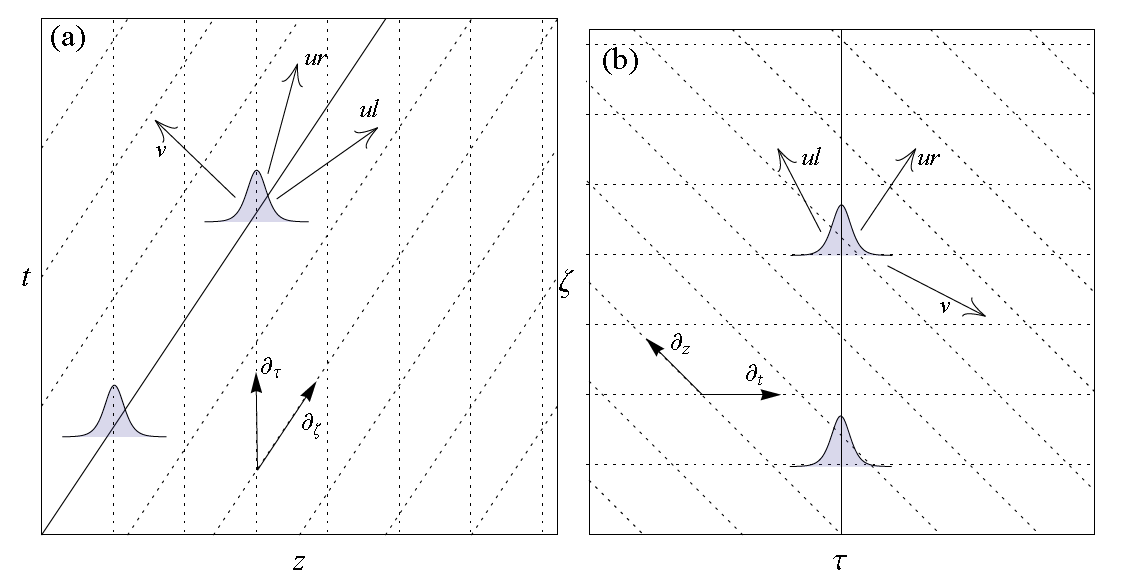
\includegraphics[scale=0.6]{F41}
	\caption{Solit\'{o}n propag\'andose en el interior de una fibra óptica descrito con las coordenadas $(x,t)$  de las ecs. (\ref{trans1})(a) y $(\zeta,\tau)$ de las ecs. (\ref{trans2}). Estas im\'agenes fueron tomadas de \citep{Robertson2011}.}\label{fig:4.1}
\end{figure}


\subsection{Linealizaci\'{o}n}
 Consideremos la propagaci\'{o}n un campo dentro de la fibra \'{o}ptica tal que su din\'{a}mica est\'{a} descrita por la ec. (\ref{NLS}). En el caso de que la radiaci\'{o}n que ingresa al material no lineal sea una onda continua, com\'{u}nmente llamada pulso de bombeo, su amplitud $\Phi(x,\tau)$ es independiente de $\tau$ en el extremo de la fibra, es decir, en $x=0$. Suponiendo que su amplitud permanece independiente de $\tau$ tambi\'{e}n en el interior de la fibra, esta onda puede ser escrita como
 \begin{equation}
 \Phi=\sqrt{n}\exp(i\kappa \beta_1 n x).
 \end{equation}
¿Ser\'{a} esta soluci\'{o}n estable ante peque\~{n}as fluctuaciones? Para responder a esta pregunta, perturbamos el estado estable ligeramente tal que
\begin{equation}\label{antz}
\Psi(x,\tau)=\Phi+\exp(i\kappa \beta_1 n x)\phi(x,\tau)=\exp(i\kappa \beta_1 n x)\Bigl[\sqrt{n}+\phi(x,\tau)\Bigr],
\end{equation} 
y examinamos la propagaci\'{o}n de la fluctuaci\'{o}n $\phi(x,\tau)$ en la ec. (\ref{NLS}).\\

Observe que
\begin{align}\label{ec:remplazo}
 \partial_{x}\Psi=&i\kappa n \beta_1\exp[i\kappa n\beta_1 x]\Bigl[\sqrt{n}+\phi(x,\tau)\Bigr]+\exp(i\kappa n\beta_1 x)\phi,\\
 \partial_{\tau}^2\Psi=&\exp(i\kappa n x)\partial_{\tau}^2\phi,\\
|\Psi|^2\Psi=&\exp(i\kappa n\beta_1 x)\Bigl[n\sqrt{n}+2n\phi+ n\phi^{*}+\sqrt{n}|\phi|^2+\sqrt{n}\phi^2\Bigr],
\end{align}
reemplazando la ec. (\ref{antz}) y los resultados obtenidos en la ec. (\ref{NLS}) y aproximando a orden lineal en la perturbaci\'{o}n $\phi$ se encuentran dos ecuaciones, la primera
\begin{equation}
i\partial_x\Phi+\kappa\beta_1|\Phi|^2\Phi=0,
\end{equation}
es la ecuaci\'{o}n que sigue la onda continua al propagarse en el interior de la fibra, la segunda
\begin{equation}\label{ec:lineal5}
i\partial_{x}\phi-\frac{\beta_2}{2}\partial_{\tau}^2\phi+\kappa\beta_1 n (\phi+\phi^{*})=0,
\end{equation}
es la ecuaci\'{o}n que sigue una fluctuaci\'{o}n lineal que se propaga sobre un campo de fondo representado por $n=|\Phi|^2$. Igual que se realiz\'{o} en el caso ac\'{u}stico, se buscan soluciones de ondas planas de la forma
\begin{equation}\label{ec:ondaplana}
\phi(x,\tau)=a_1\exp[i(\beta x-\omega \tau)]+a_2^*\exp[-i(\beta x-\omega \tau)].
\end{equation}
Primero calculemos los t\'{e}rminos
\begin{align}\label{ec:rem2}
\nonumber \partial_{x}\phi&=ia_1\beta\exp[i(\beta x-\omega \tau)]-i\beta a_2^*\exp[-i(\beta x-\omega \tau)]\\
\nonumber \partial_{\tau}^2\phi&=-\omega^2a_1\exp[(\beta x-\omega \tau)]-\omega^2a_2^*\exp[-i(\beta x-\omega \tau)].
\end{align}
Reemplazando las ecs. (\ref{ec:ondaplana}) y ecs. (\ref{ec:rem2}) en (\ref{ec:lineal5}) se obtiene

\begin{align}
\kappa&\beta_1 n\Bigl((a_1+a_2)\exp[(\beta x-\omega \tau)]+(a_1^*+a_2^*)\exp[-(\beta x-\omega \tau)]\Bigr)\\
\nonumber&-\frac{\beta_2}{2}\left(-\omega^2 a_1\exp[(\beta x-\omega \tau)]-\omega^2a_2^*\exp[-(\beta x-\omega \tau)]\right) \\
\nonumber& -\beta a_1\exp[(\beta x-\omega \tau)]+\beta a_2^*\exp[-(\beta x-\omega \tau)]=0.
\end{align}
Separando en t\'{e}rminos linealmente independientes o por frecuencias negativas y positivas se tiene, para $\exp[i(\beta x-\omega \tau)]$
\begin{equation}
-\beta a_1+\frac{\beta_2}{2}\omega^2 a_1+\kappa\beta_1 n a_1+\kappa\beta_1 n a_2=0,
\end{equation}
y para $\exp[-i(\beta x-\omega \tau)]$
\begin{equation}
\beta a_2^* +\frac{\beta_2}{2}\omega^2 a_2^*+\kappa\beta_1 n a_2^*+\kappa\beta_1 n a_1^*=0.
\end{equation}
Reescribiendo lo anterior en forma matricial
\begin{equation}
\begin{pmatrix}
-\beta+\displaystyle \frac{\beta_2}{2}\omega^2+\kappa\beta_1 n &\kappa\beta_1 n\\
\kappa\beta_1 n &\beta+ \displaystyle\frac{\beta_2}{2}\omega^2+\kappa\beta_1 n
\end{pmatrix}\begin{pmatrix}
a_1\\
a_2
\end{pmatrix}=\begin{pmatrix}
0\\
0  
\end{pmatrix}.
\end{equation}
Los t\'{e}rminos por fuera de la diagonal mezclan modos de frecuencia negativa con modos de frecuencia positiva que es un ingrediente necesario para el proceso Hawking. El anterior problema tiene soluciones no triviales cuando el determinante es nulo, lo cual se cumple cuando
\begin{align}
\beta^2&=\beta_2\kappa\beta_1 n\omega^2+\frac{\beta_2^2}{4}\omega^4,\\
\beta^2&=\frac{\omega^2}{c^2}\Bigl(b_1^2+b_2\omega^2\Bigr),\label{ec:gaona}
\end{align}
donde $b_1^2= c^2 \beta_2\kappa \beta_1 n$ y $b_2=c^2\beta_2^2/4$ caracterizan la relaci\'{o}n de dispersi\'{o}n a partir de constantes propias del material y la velocidad de grupo del pulso que entra al mismo. Este tipo de dispersi\'{o}n se conoce en la literatura como dispersi\'{o}n normal\footnote{Un material tiene dispersi\'{o}n normal cuando la velocidad de grupo ($\partial \omega/\partial \beta$) para un modo decrece a medida que la frecuencia crece.} y ser\'{a} una de las diferencias principales al comparar el an\'{a}logo \'{o}ptico con el ac\'{u}stico.\\
La ec. (\ref{ec:gaona}) es la ec. ($9$) en \cite{GaonaReyes2017}. En este art\'{i}culo, $b_1$ y $b_2$ son los par\'{a}metros que ajustan la mejor curva alrededor de la frecuencia de horizonte para la relaci\'{o}n de dispersi\'{o}n encontrada experimentalmente para un material como las fibras de cristal fot\'{o}nico (PCF).\\
\begin{figure}\centering
	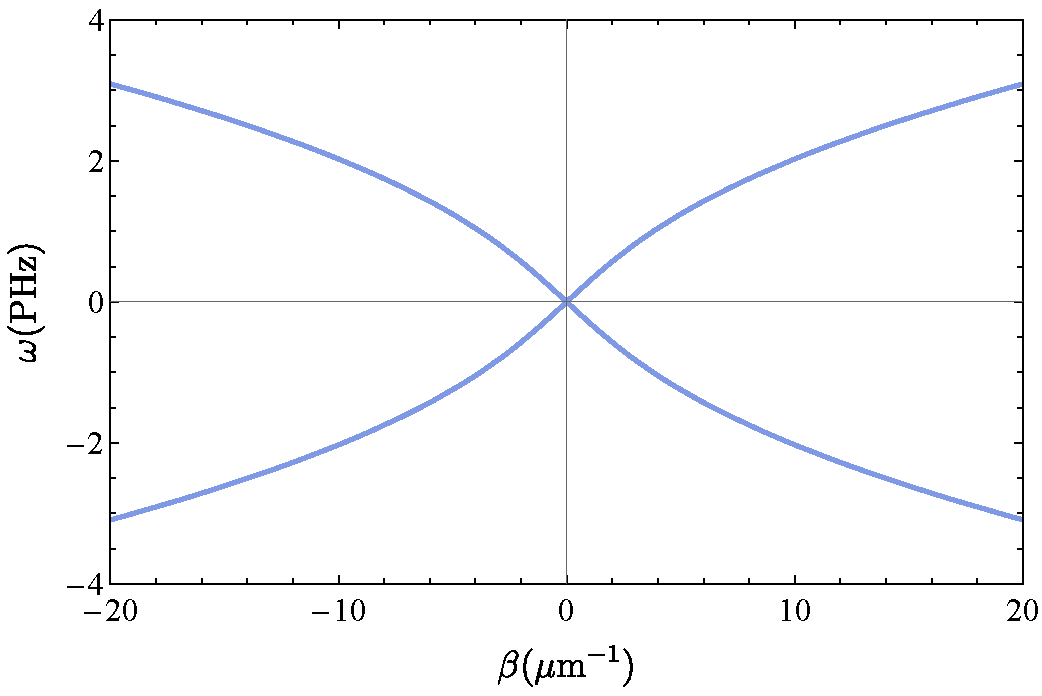
\includegraphics[scale=0.6]{f42}
	\caption{Relaci\'{o}n de dispersi\'{o}n normal dada por la ec. (\ref{ec:gaona}).}\label{fig:labdis}
\end{figure}
\subsection{Relaci\'{o}n de dispersi\'{o}n}\label{normaneg}
El prop\'{o}sito es encontrar la frecuencia $\omega'$ en el marco com\'{o}vil cuando se considera el efecto de una perturbaci\'{o}n en el \'{i}ndice de refracci\'{o}n\footnote{Es com\'{u}n definir el \'{o}ptica, el n\'{u}mero de onda en t\'{e}rminos del \'{i}ndice de refracci\'{o}n: $\beta=n(\omega)\omega/c$, tal que un cambio en el \'{i}ndice, ocasiona que el n\'{u}mero de onda se vea afectado de la forma  $\beta=(n(\omega)+\delta n)\omega/c$.}. Usando la relaci\'{o}n de efecto Doppler en la ec. (\ref{ec:doppler}) e ignorando por ahora el factor de Lorentz, se puede escribir 
\begin{align}
\omega'=\omega-u(\beta+\frac{\omega}{c}\delta n)
=\omega-u\frac{\omega}{c}\Bigl(\sqrt{b_1^2+b_2\omega^2}+\delta n\Bigr).
\end{align}
Reorganizando la \'{u}ltima ecuaci\'{o}n se encuentra la relaci\'{o}n de dispersi\'{o}n
\begin{equation}\label{ec:disoptica}
\Bigl[W'-W\upsilon(\tau)\Bigr]^2=W^2+\frac{W^4}{\Omega_0^2},
\end{equation}
donde $W=b_1\omega$, las constantes $W'$ y $\Omega_0$ son dadas por las relaciones $W'=\omega'n_{g0}$, $\Omega^2_0=b_1^4/b_2$ y definimos la \textit{velocidad} del medio  \'{o}ptico como $\upsilon(\tau)=(-n_{g0}+\delta n)/b_1$ que es el cambio del \'{i}ndice de refracci\'{o}n escalado por $b_1$, llamamos a esta cantidad adimensional \textit{velocidad}, en analog\'{i}a con el caso ac\'{u}stico. Aqu\'{i} hemos empleado la definici\'{o}n usual del \'{i}ndice de grupo $n_{g0}=c/u$. Con esto surge la pregunta, ¿qu\'{e} es lo que fluye en el medio? Observe que aqu\'{i} realmente no hay un medio en movimiento, el cambio de velocidad se debe ahora a la dispersi\'{o}n. En la secci\'{o}n \ref{OBHL} el perfil de velocidades es nuevamente  negativo, y con \'{e}ste se analizar\'{a} la configuraci\'{o}n de l\'{a}ser \'{o}ptico de agujeros negros en la siguiente secci\'{o}n. Reorganizar la relaci\'{o}n de dispersi\'{o}n de la ec. (\ref{ec:disoptica}) nos permite mostrar que tiene la misma estructura que el caso ac\'{u}stico con BEC. Para no saturar la notaci\'{o}n en lo que sigue, absorberemos la constante $n_{g0}$ en $\omega'$ teniendo as\'{i} $W'\rightarrow\omega'$ y haremos sin p\'{e}rdida de generalidad $b_1=1$, de que aqu\'{i} en adelante la relaci\'{o}n de dispersi\'{o}n en el caso \'{o}ptico ser\'{a}
\begin{equation}\label{disperoptica}
\Bigl[\omega'-\omega v(\tau)\Bigr]^2=\omega^2+\frac{\omega^4}{\Omega_0^2},
\end{equation}
toda la informaci\'{o}n de la no linealidad del sistema est\'{a} contenida en $\Omega_0$, que representa la escala de dispersi\'{o}n del mismo modo que $k_0$ en el caso ac\'{u}stico.\\

En el caso ac\'{u}stico, donde $\omega$ era la frecuencia de una perturbaci\'{o}n generada en el sistema, \'{e}sta se mantiene constante en el marco de laboratorio. En el caso \'{o}ptico, la frecuencia que se mantiene constante es $\omega'$ que mide las oscilaciones de la perturbaci\'{o}n en el marco com\'{o}vil y es la raz\'{o}n fundamental por la cual trabajar dicho marco.\\

Por \'{u}ltimo, dado que la relaci\'{o}n de dispersi\'{o}n es cu\'{a}rtica en $\omega$, indica que un modo a $\omega'$ fija es
\begin{align}\label{ec:ondaplana2}
\phi=\exp[-i\omega'\zeta]\sum_j A_j\exp[-i\omega_j \tau].
\end{align}

Alternativamente, es \'{u}til derivar la misma relaci\'{o}n de dispersi\'{o}n a partir de una acci\'{o}n
\begin{equation}\label{accion}
S_{\phi}=\int d\zeta \mathfrak{L}=\frac{\epsilon_0}{2}\int d\zeta d\tau \Bigl\{[(\partial_{\zeta}-v(\tau)\partial_{\tau})\phi]^2+\phi\left(\partial_{\tau}^2-\frac{\partial_{\tau}^4}{\Omega_0}\right)\phi\Bigr\},
\end{equation}

aplicando las ecuaciones de Euler-Lagrange se produce la siguiente ecuación de movimiento
\begin{equation}
[\partial_{\zeta}-\partial_{\tau}v(\tau)][\partial_{\zeta}-v(\tau)\partial_{\tau}]\phi=\left(\partial_{\tau}^2-\frac{\partial_{\tau}^4}{\Omega_0}\right)\phi.
\end{equation}
Suponiendo que el perfil de velocidades es constante en cierta regi\'{o}n del espacio se pueden proponer soluciones de ondas planas ec. (\ref{ec:ondaplana2}) y encontrar la relaci\'{o}n de dispersi\'{o}n dada en la ec. (\ref{disperoptica}).\\

Cuando el campo escalar $\phi$ en la acci\'{o}n ec. (\ref{accion}) es complejo, su lagrangiana $\mathfrak{L}$  es invariante con respecto a las
transformaciones de norma $\phi'=\exp[i\lambda]\phi$. Por tanto existe una corriente conservada, de tal manera que su componente $\zeta$  puede usarse para definir el siguiente producto interno
\begin{equation}\label{productointerno}
(\phi_1,\phi_2)=\frac{i\epsilon_0c^2}{u\hbar}\int d\tau \ [\phi_1^*(\partial_{\zeta}-v(\tau)\partial_{\tau})\phi_2-\phi_2(\partial_{\zeta}-v(\tau)\partial_{\tau})\phi_1^*],
\end{equation}
el cual satisface $\partial_{\zeta}(\phi,\phi)=0,$ que es la conservaci\'{o}n de la norma. Este producto interno coincide con el definido por \cite{philbin2008fiber} y \cite{Robertson2011} excepto por el factor $-1$. Esta convención suele ser elegida para que los signos de la norma y frecuencia coincidan en el marco del laboratorio. 


\section{Configuraci\'{o}n de un l\'{a}ser \'{o}ptico de agujeros negros (OBHL)}\label{OBHL}
En el cap\'{i}tulo \ref{cap2} observamos que en sistemas ac\'{u}sticos la radiaci\'{o}n de Hawking an\'{a}loga confinada en el interior de dos horizontes sufre un proceso de autoamplificaci\'{o}n. ¿Ser\'{a} posible obtener el mismo proceso de amplificaci\'{o}n para la radiaci\'{o}n cambiando de un sistema ac\'{u}stico a  uno \'{o}ptico? La respuesta es tratada en \cite{Faccio2012} y \cite{GaonaReyes2017} y se describir\'{a} brevemente aqu\'{i}. Se requiere una cavidad óptica resonante que actúe como amplificador y una relaci\'{o}n de dispersi\'{o}n normal como la encontrada en la ec. (\ref{ec:gaona}). El análogo gravitatorio a esta cavidad podría ser el espacio-tiempo entre los horizontes de eventos de un agujero negro y un agujero blanco. Sin embargo, en lugar de agujeros astrof\'{i}sicos se podrían utilizar sus análogos. Con una fibra óptica se pueden fabricar tanto agujeros negros (BH) ópticos como agujeros blancos (WH). El análogo óptico para horizontes más prometedor fue propuesto por \cite{philbin2008fiber} en pulsos de luz propag\'andose en una fibra óptica; donde los horizontes se obtienen en las ondas de choque que aparecen en los frentes de pulsos ópticos intensos en un material refractivo no lineal. Cabe destacar que con esta forma de crear horizontes en los análogos ópticos s\'{o}lo se ha podido medir la RH de forma estimulada \citep{drori2019observation}, pero a\'{u}n contin\'{u}a el reto de verificar el proceso espontáneo que es realmente el mecanismo de Hawking. El láser óptico de agujeros negros (OBHL) solo puede funcionar si la predicción de Hawking es correcta, lo que significa que si en un laboratorio se logra fabricar este tipo de láser se habrá demostrado la existencia de la RH en un experimento an\'{a}logo.\\

Para crear los horizontes en \'{o}ptica se envía un \textit{pulso de bombeo} a través de un material óptico no lineal en el que el índice de refracción depende de la intensidad del pulso que se propaga en el medio. Esta dependencia es de la forma

\begin{equation}\label{n2}
n(\omega,\tau)=n_{0}(\omega)+n_2I(\tau)=n_{0}(\omega)+\delta n(\tau).
\end{equation}

Por tanto, el índice efectivo $n(\omega,\tau)$ depende tanto de la posici\'{o}n del pulso como de la frecuencia. Si adem\'{a}s se env\'{i}a un segundo pulso denominado \textit{pulso de prueba} en la misma direcci\'{o}n que el primero y con una velocidad de grupo mayor pero cercana a la velocidad de grupo del pulso de bombeo, el segundo pulso al acercarse al primero disminuir\'{a} su velocidad ya que siente un \'{i}ndice de refracci\'{o}n que aumenta a medida que se propaga. Esta disminuci\'{o}n en la velocidad puede ser tal que el segundo pulso nunca adelante al primero, cre\'{a}ndose un an\'{a}logo de WH. Para un observador sobre el pulso de bombeo el pulso de prueba se acerca a \'{e}l pero nunca lo alcanza, i.e., existe una regi\'{o}n en el espacio que es imposible de alcanzar para el pulso de prueba. En la figura \ref{fig:analogoopticoWH} se muestra el comportamiento de los pulsos para un observador en los marcos de laboratorio y com\'{o}vil que se mueve con el pulso de bombeo.\\

De forma similar se puede crear el an\'{a}logo de BH cuando el pulso de prueba se envia en direci\'{o}n opuesta al pulso de bombeo. Con este m\'{e}todo el pulso de bombeo genera ambos horizontes, el WH en el frente anterior y el BH en el frente posterior del pulso, en la figura \ref{fig:analogoWHBH} se muestra esta situaci\'{o}n.

\begin{figure}
   \centering
   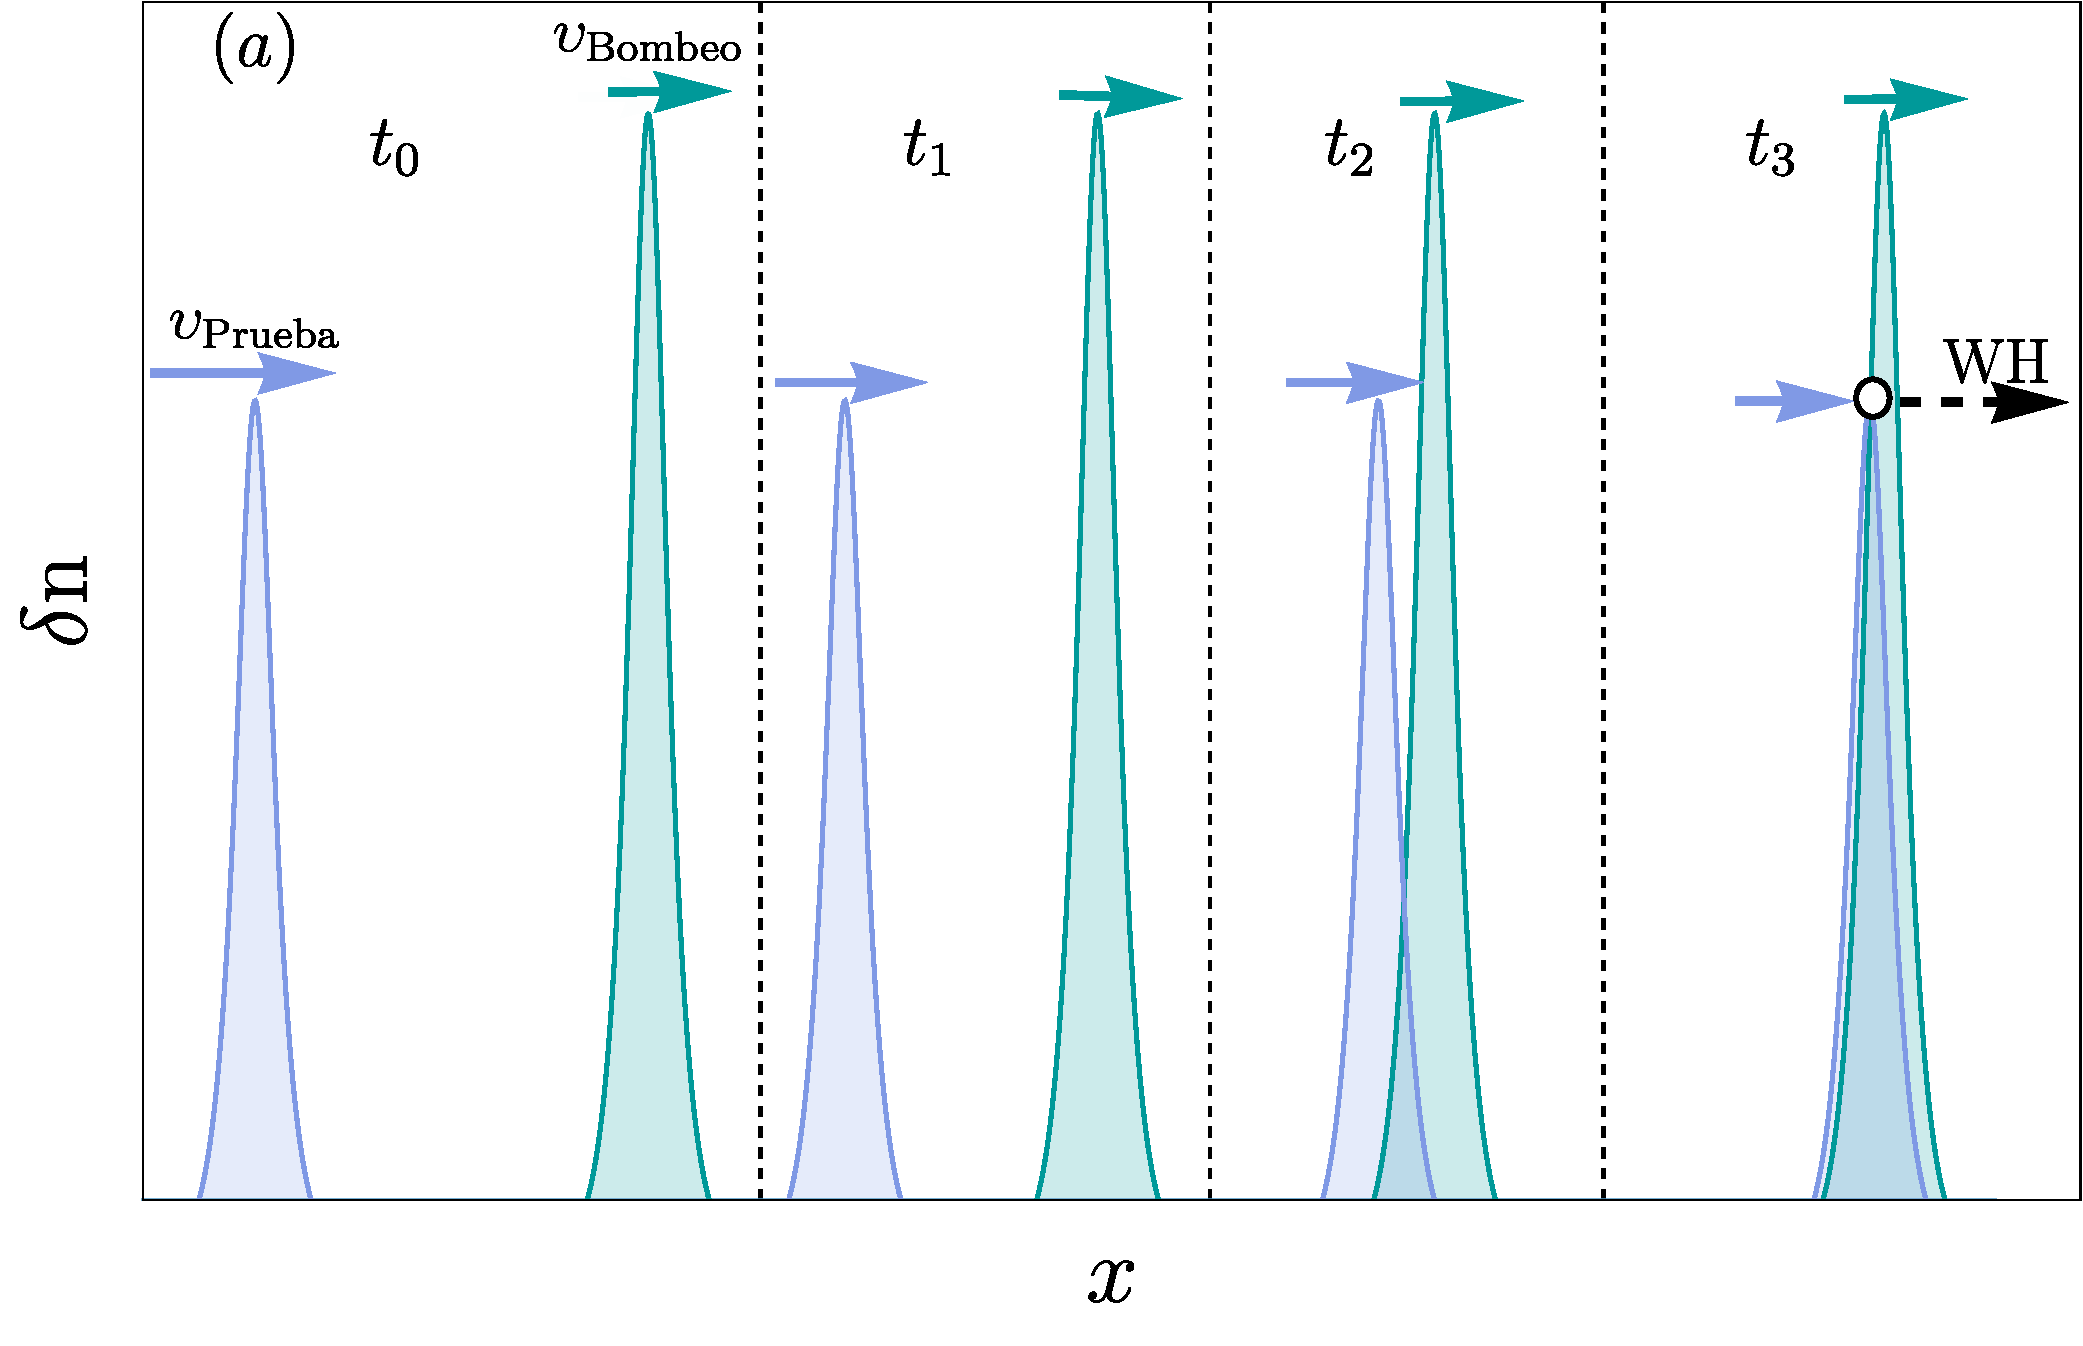
\includegraphics[height=4.7cm]{final43a.pdf}%
   \hspace{0.1cm}% add some horizontal spacing
   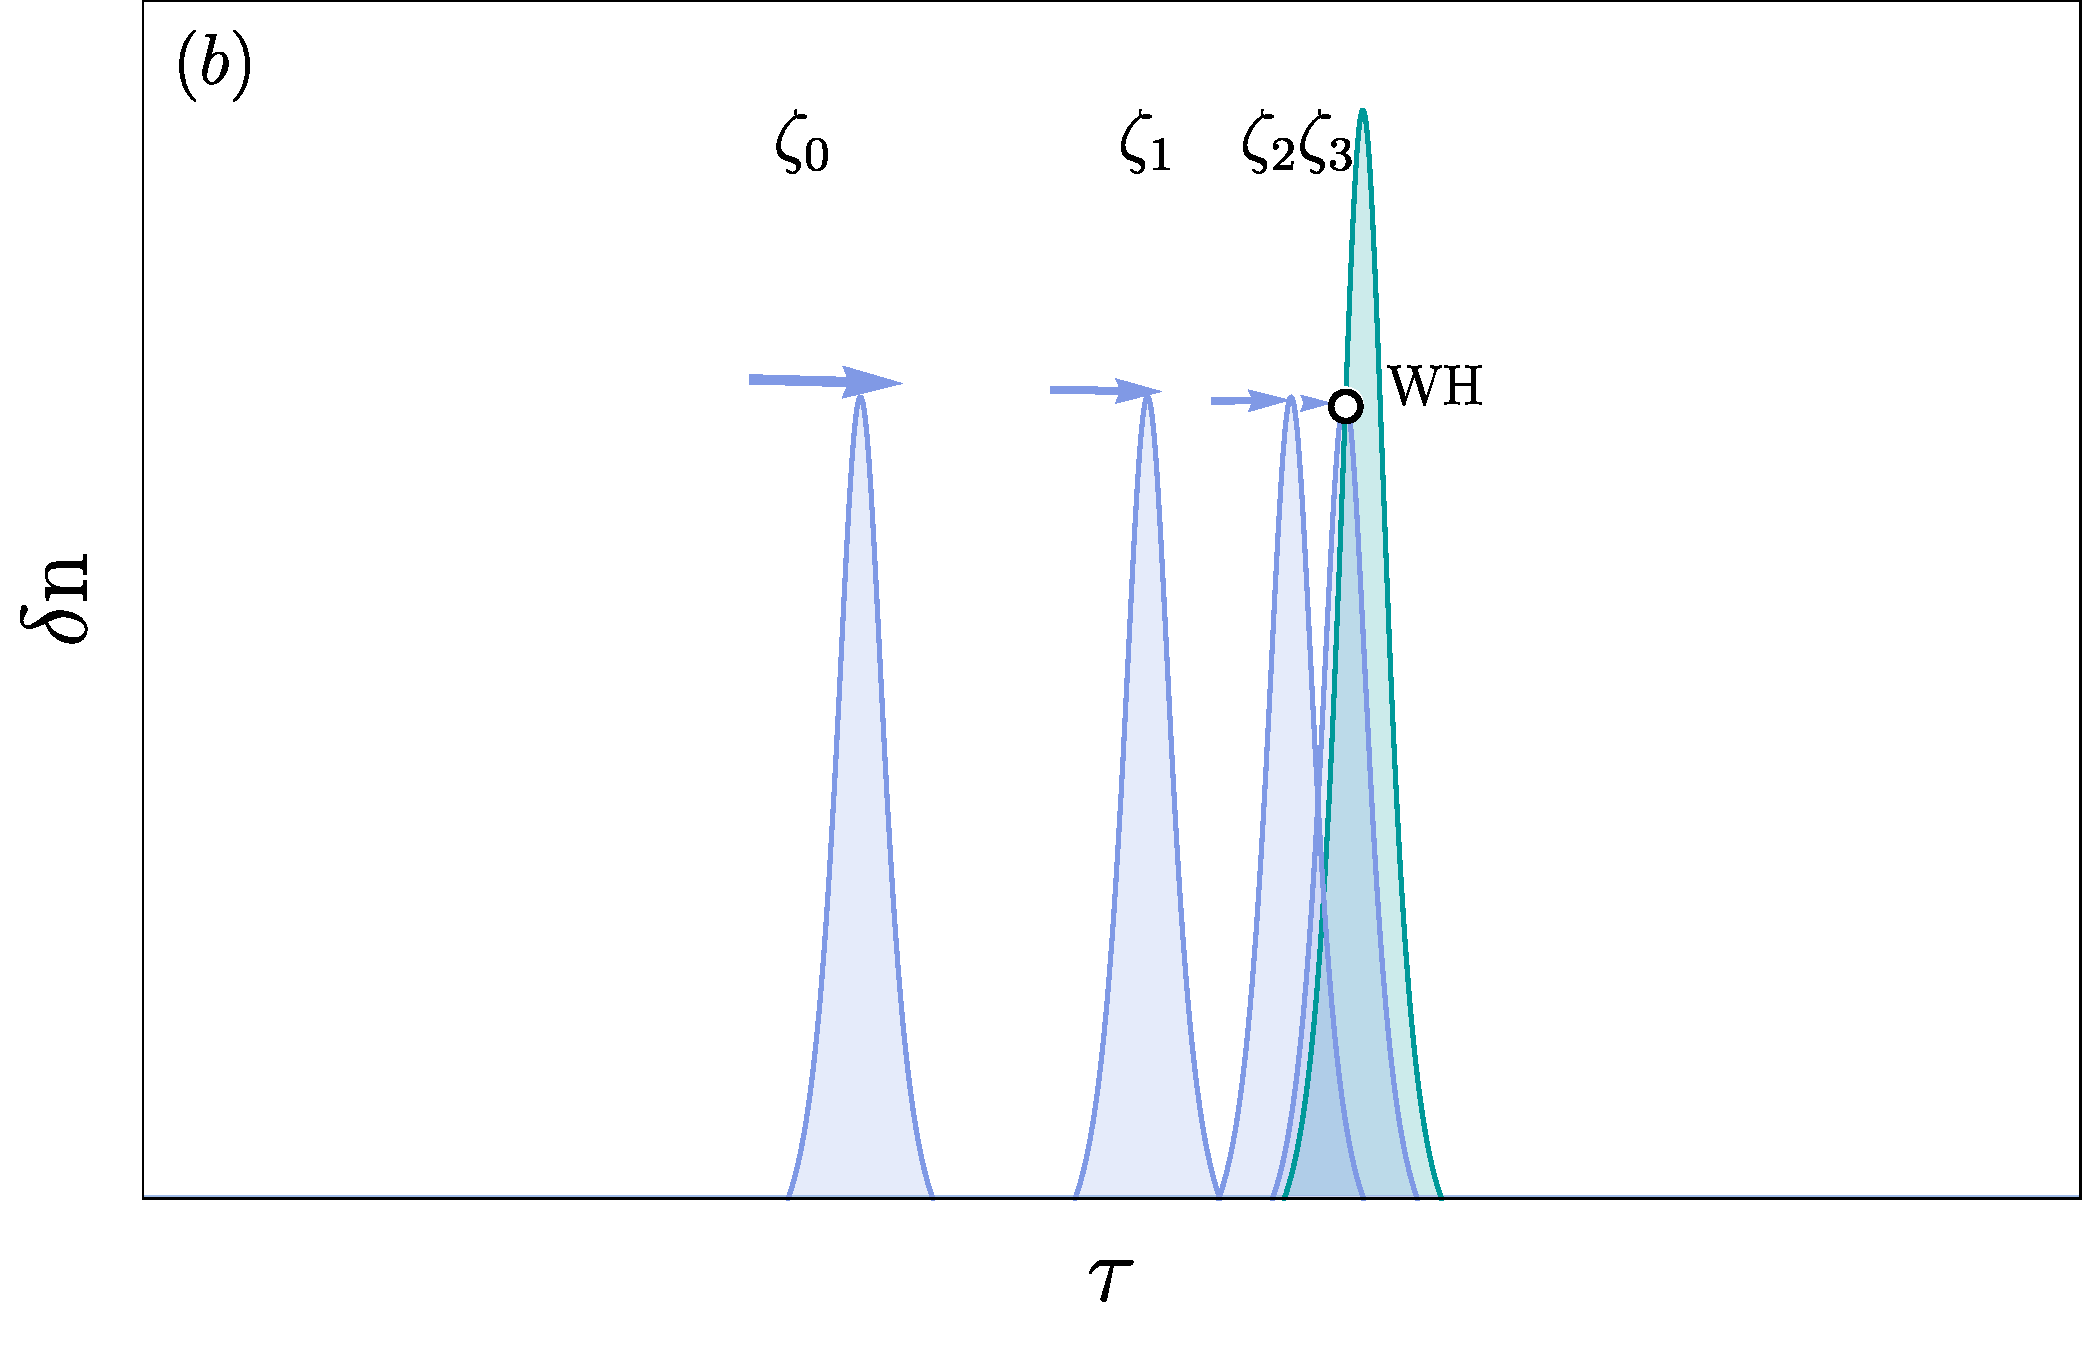
\includegraphics[height=4.7cm]{final43b.pdf}%
   \caption{Comportamiento para el pulso de prueba al acercarse al pulso de bombeo visto desde el marco de laboratorio (a) y desde el marco com\'{o}vil (b).} 
   \label{fig:analogoopticoWH}
\end{figure}



\begin{figure}
   \centering
   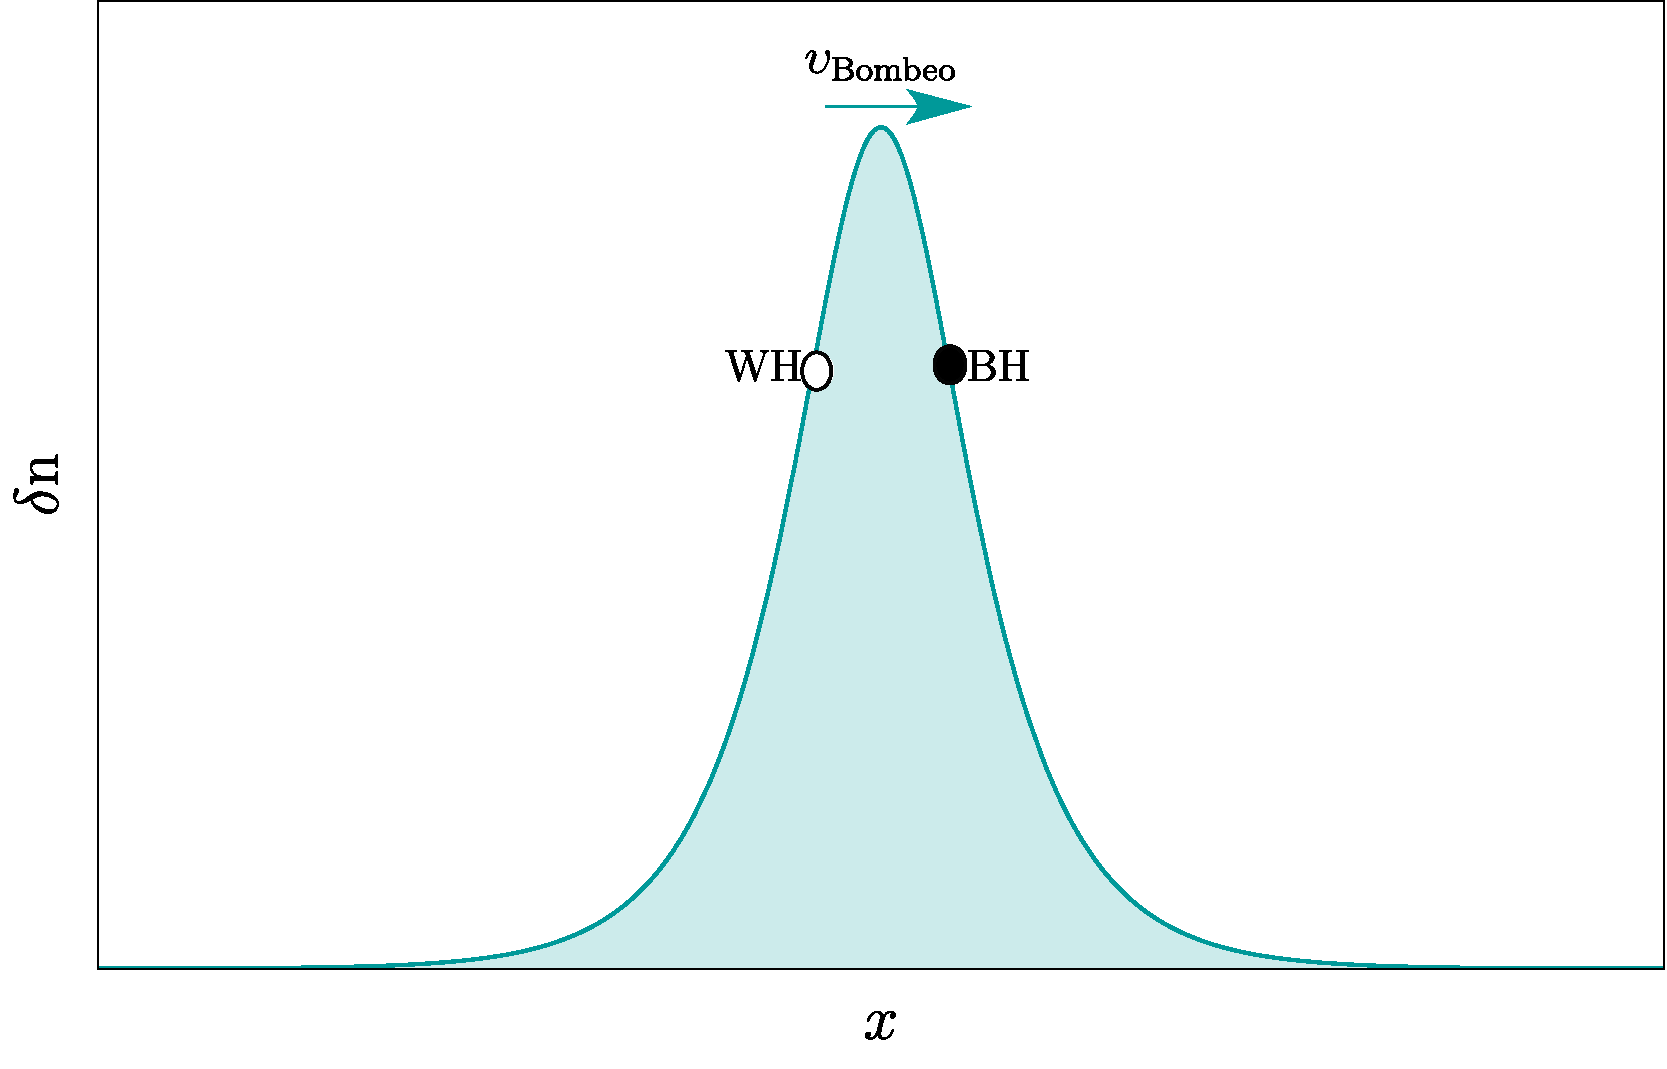
\includegraphics[height=4.7cm]{F45.pdf}%
   \caption{Un pulso de prueba propag\'{a}ndose en el interior del material no lineal genera un WH en el frente anterior y el BH estado en el frente posterior del pulso .} 
   \label{fig:analogoWHBH}
\end{figure}

Ahora que sabemos c\'{o}mo crear horizontes por medio de pulsos \'{o}pticos es posible construir una cavidad para la configuraci\'{o}n de OBHL. Esta se crea env\'iando dos pulsos con las mismas caracter\'{i}sticas en el interior de la fibra \'{o}ptica, los pulsos deben de estar separados uno de otro una distancia $\text{L}_c$ o un tiempo de retardo $\tau_c$. La cavidad ser\'{a} entonces la regi\'{o}n entre los pulsos que se mueven en el interior de la fibra con la velocidad que se propagan los pulsos tal como se muestra en la figura \ref{fig:cavidadlab}(a). En un marco que se mueve con los pulsos la cavidad permanece en reposo. Matem\'{a}ticamente esto se logra bajo el cambio de coordenadas dado en la ec. (\ref{trans2}). Observe que el orden de los horizontes se intercambia tal como se muestra en la figura \ref{fig:cavidadlab}(b).\\

La cavidad es entonces una regi\'{o}n entre un WH y BH que por simplicidad consideramos con $\delta n=0$ mientras que el exterior a la cavidad ser\'{a} la regi\'{o}n con $\delta n=\delta n_{\text{max}}$.

\begin{figure}
   \centering
   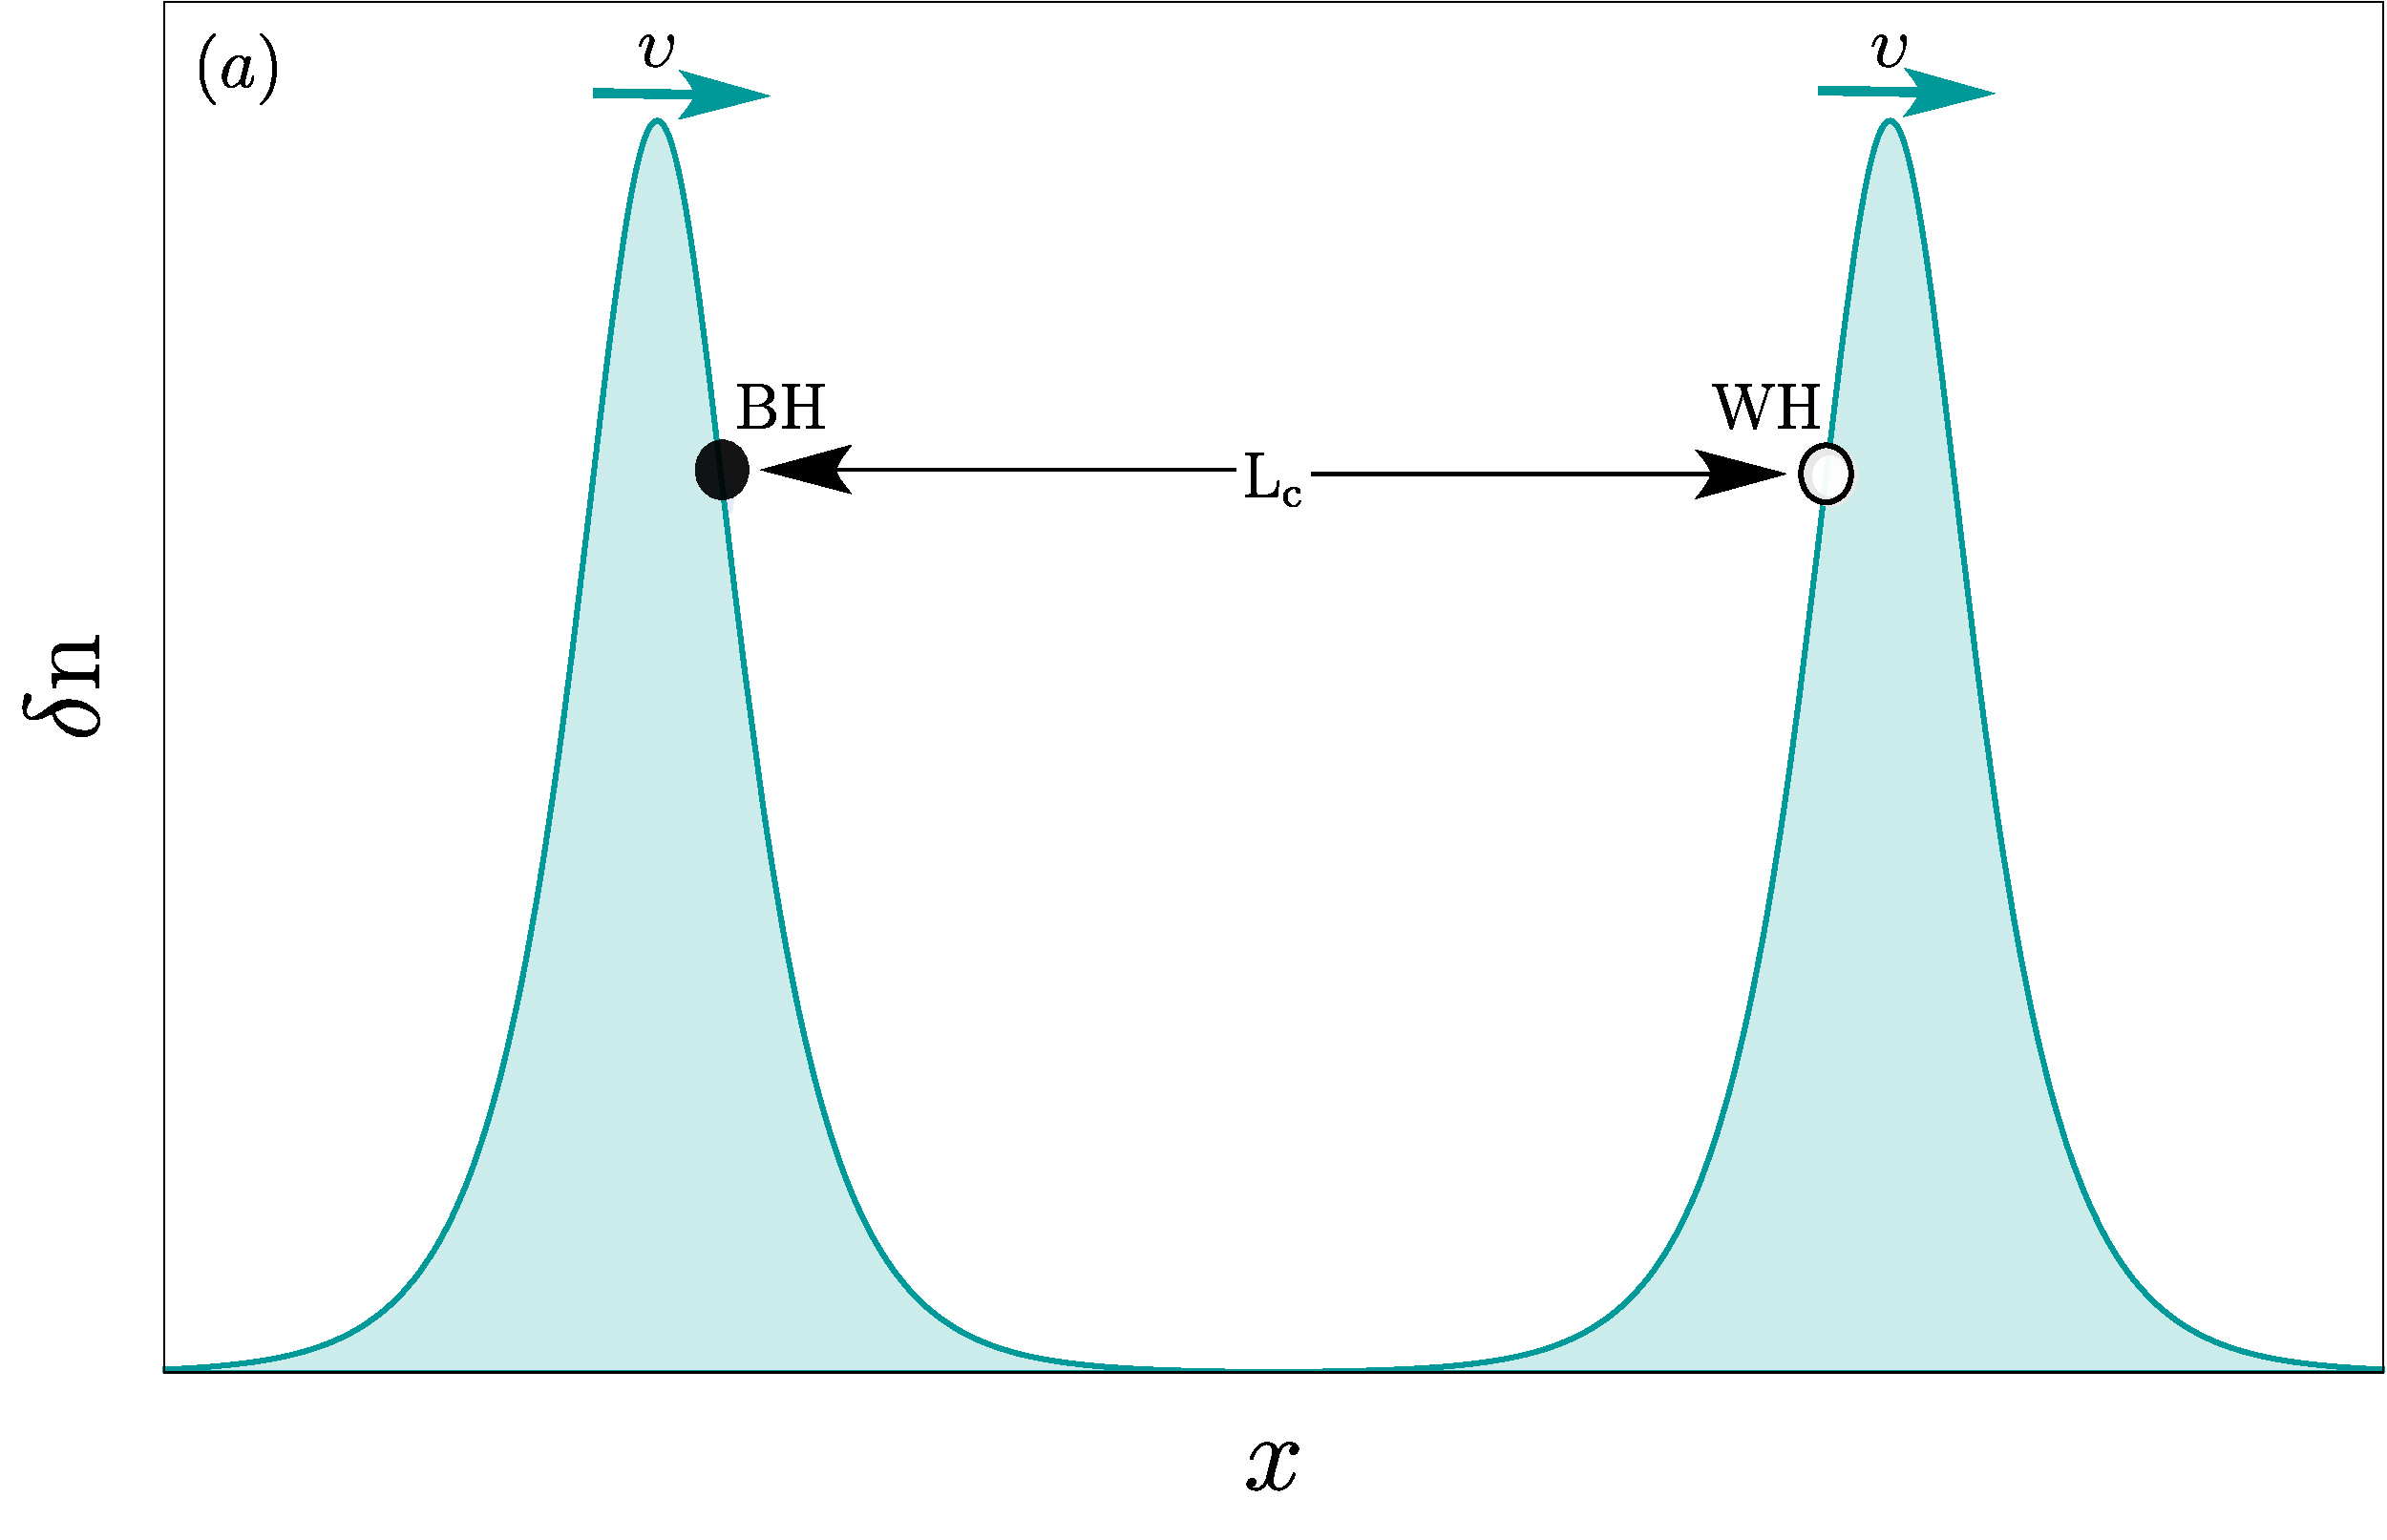
\includegraphics[height=4.7cm]{F44a.pdf}%
   \hspace{0.1cm}% add some horizontal spacing
   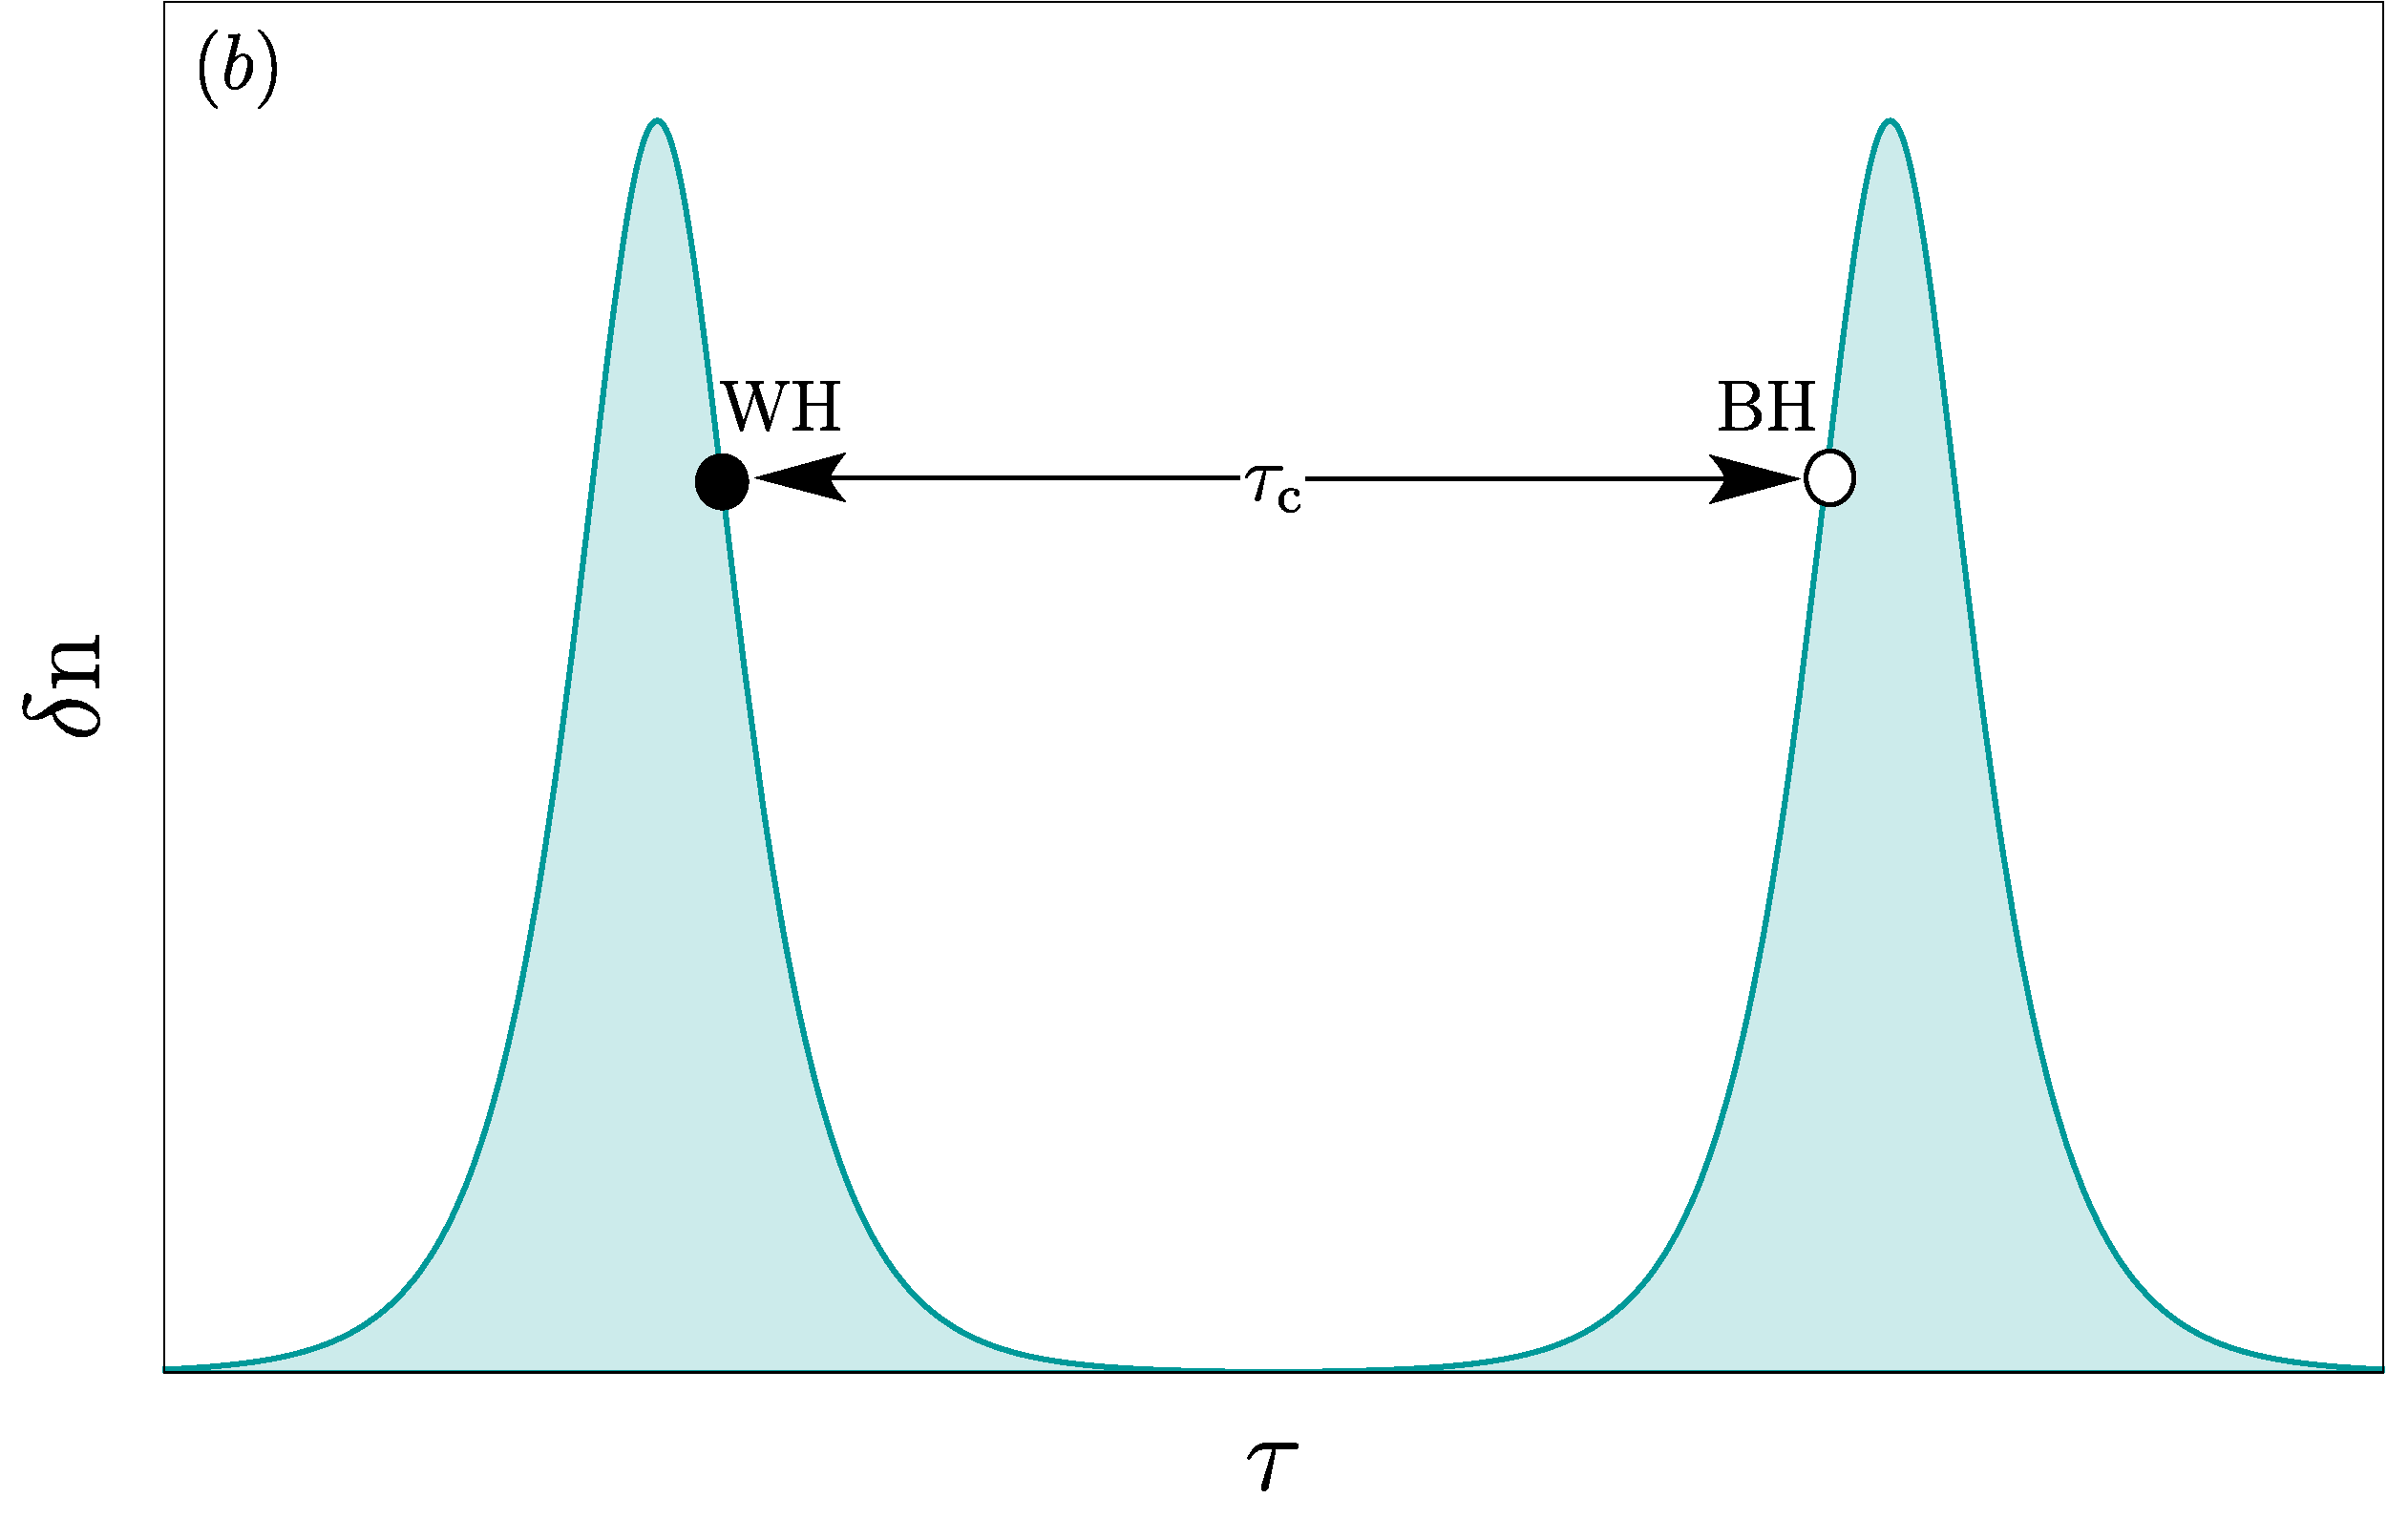
\includegraphics[height=4.7cm]{F44b.pdf}%
   \caption{Cavidad formada por dos solitones vista en el marco de laboratorio (a) con coordenadas ($x,t$) y desde el marco com\'{o}vil (b) dado por las coordenadas ($\tau,\zeta$). Observe que en el marco com\'{o}vil el orden de los horizontes se cambia y esto se debe al cambio de coordenadas dado en la ec. (\ref{trans2}).} 
   \label{fig:cavidadlab}
\end{figure}

\begin{figure}
   \centering
   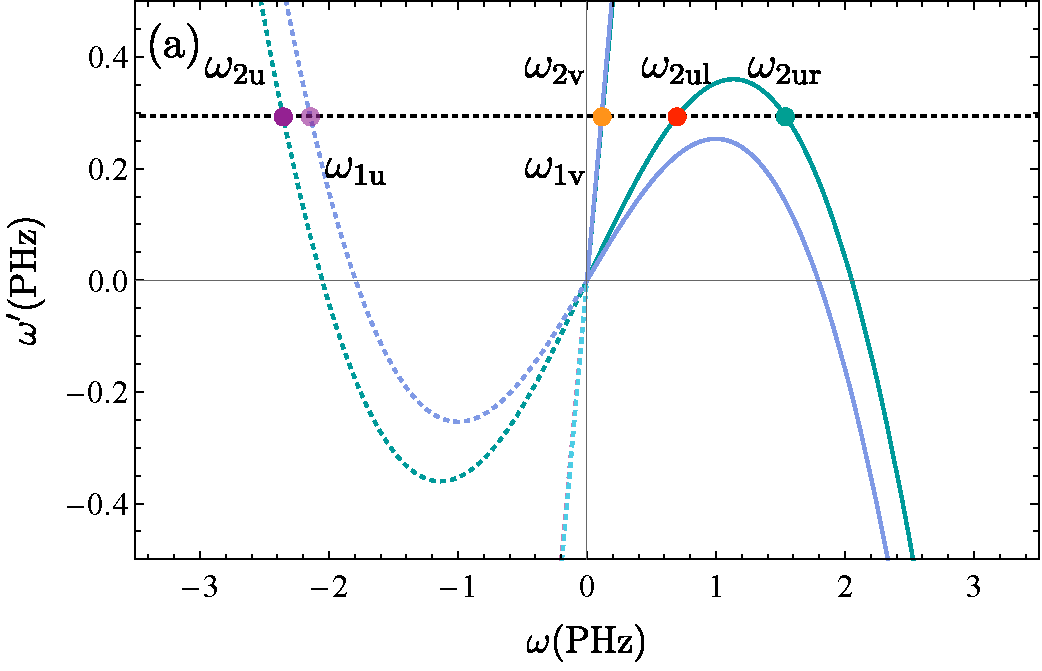
\includegraphics[height=5cm]{f52a.pdf}%
   \hspace{0.1cm}% add some horizontal spacing
   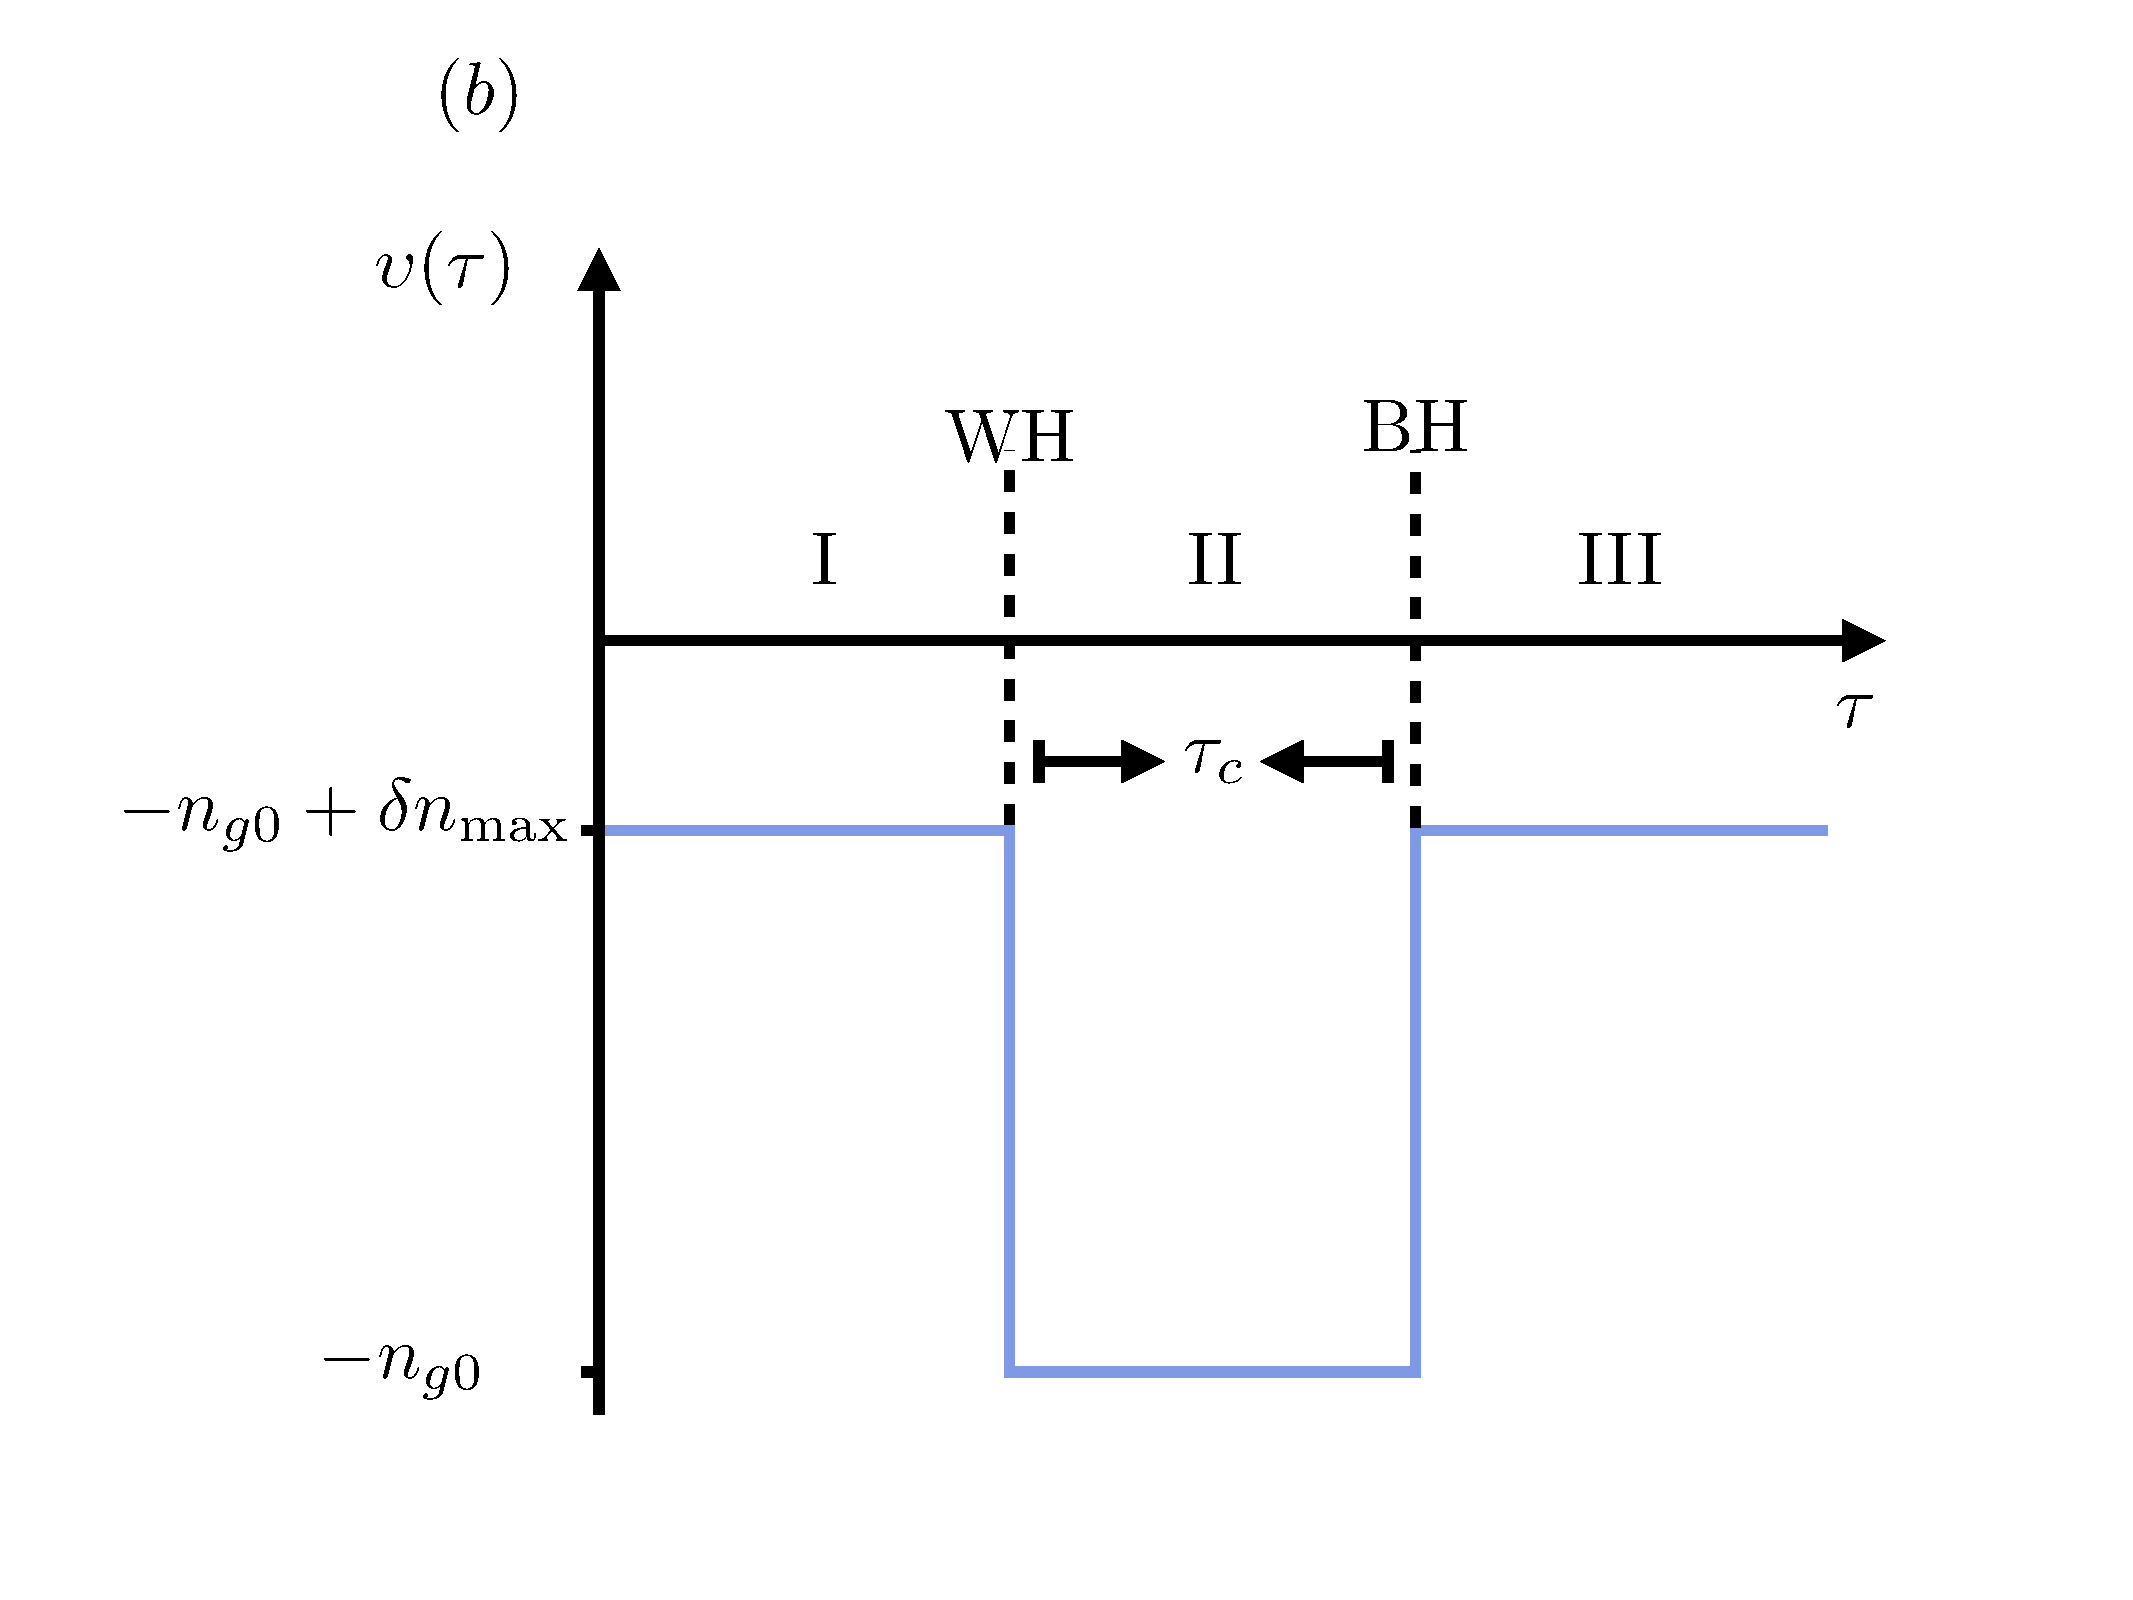
\includegraphics[height=5cm]{jdc2-2.pdf}%
   \caption{(a) Relaci\'{o}n de dispersi\'{o}n en el marco com\'{o}vil. (b) Perfil de velocidad simplificado.} 
   \label{fig:ultima}
\end{figure}

De la ec. (\ref{ec:disoptica}) que es la relaci\'{o}n de dispersi\'{o}n que sigue una fluctuaci\'{o}n al propagarse en un medio no lineal y con dispersi\'{o}n, vemos que al aplicarse a la configuraci\'{o}n de OBHL la cantidad $\upsilon(\tau)$ define dos regiones: una regi\'{o}n lenta que es el exterior de la cavidad y donde las fluctuaciones sienten un cambio del \'{i}ndice de refracci\'{o}n dado por $\upsilon(\tau)=-n_{g0}+\delta n_{\text{max}}$ y una regi\'{o}n r\'apida donde la fluctuaci\'{o}n se mueve a la velocidad de los pulsos que crearon la cavidad porque sienten que $\upsilon(\tau)=-n_{g0}$. Observe que $\upsilon(\tau)$ representa un perfil de velocidad negativo y adimensional del medio no lineal y las fluctuaciones \'{o}pticas se propagan sobre este medio en movimiento tal como se estudio en el cap\'{i}tulo \ref{cap2} con las fluctuaciones ac\'{u}sticas propag\'{a}ndose sobre un fluido en movimiento. Se presenta en la figura \ref{fig:ultima}(a) la relaci\'{o}n de dispersi\'{o}n de la ec. (\ref{ec:disoptica}) cuando $\upsilon(\tau)$ solo toma dos posibles dados en la figura \ref{fig:ultima}(b), que es el perfil de velocidades m\'{a}s simple para analizar la din\'{a}mica de una fluctuaci\'{o}n en la configuraci\'{o}n de OBHL, que ser\'{a} el tema a tratar en el cap\'{i}tulo \ref{cap5}.\\

Por \'{u}ltimo, la construcci\'{o}n de la cavidad \'{o}ptica se puede realizar tambi\'{e}n cambiando los dos solitones por un solit\'{o}n oscuro o \textit{dark soliton} \citep{weiner1988experimental}, el cual permite reproducir dos regiones con un \'{i}ndice de refracci\'{o}n diferente.\\
